\setcounter{excounter}{1}
\setcounter{examplecounter}{1}
\chapter{Advanced Object-Oriented Programming}
\label{chapter-advanced-oop} % Always give a unique label
% use \chaptermark{}
% to alter or adjust the chapter heading in the running head

\abstract*{Each chapter should be preceded by an abstract (no more than 200 words) that summarizes the content. The abstract will appear \textit{online} at \url{www.SpringerLink.com} and be available with unrestricted access. This allows unregistered users to read the abstract as a teaser for the complete chapter.
Please use the 'starred' version of the new \texttt{abstract} command for typesetting the text of the online abstracts (cf. source file of this chapter template \texttt{abstract}) and include them with the source files of your manuscript. Use the plain \texttt{abstract} command if the abstract is also to appear in the printed version of the book.}

\abstract{Each chapter should be preceded by an abstract (no more than 200 words) that summarizes the content. The abstract will appear \textit{online} at \url{www.SpringerLink.com} and be available with unrestricted access. This allows unregistered users to read the abstract as a teaser for the complete chapter. \newline\indent
Please use the 'starred' version of the new \texttt{abstract} command for typesetting the text of the online abstracts (cf. source file of this chapter template \texttt{abstract}) and include them with the source files of your manuscript. Use the plain \texttt{abstract} command if the abstract is also to appear in the printed version of the book.}

\section{Interfaces}

Interfaces are a way of grouping classes together by a ubiquitous behavior. 
We have worked with interfaces before without acknowledging their properties as an interface.
For example, the \ttt{Comparable} interface is implemented by classes that we want to be able to inhibit ``comparable'' behavior. 
In particular, there is a single method that must be implemented by any class that implements the \ttt{Comparable} interface: \ttt{compareTo}. 
The \ttt{compareTo} method receives a single parameter of the same type as the class that implements the \ttt{Comparable} interface, and returns an integer. 
Said integer is negative if \ttt{this} object instance is less than the passed argument, zero if \ttt{this} object instance is equal to the passed argument, and positive if \ttt{this} object instance is greater than the passed argument.

So, by having a class implement the \ttt{Comparable} interface, we group it into that subset of classes that are, indeed, comparable. 
Doing so implies that these classes have an ordering and are sortable in, for example, a Java collection. 

In addition to the \ttt{Comparable} interface, we have worked with the \ttt{List}, \ttt{Queue}, and \ttt{Map} interfaces, which all have a set of methods that must be implemented by any class that implements the interface. 
Recall that \ttt{ArrayList} and \ttt{LinkedList} are ``kinds of'' \ttt{List} objects, and this interface describes several methods that all lists, by definition, must override.\footnote{Here we clarify that ``kind of,'' in this context, means to implement the \ttt{List} interface.} 
To \emph{override} a method means that we provide a new implementation of the method that is different from the default implementation provided by the interface.

\subsection*{Defining an Interface}

\myexample{Imagine that we want to design an interface that describes a shape.} 
All (two-dimensional) shapes have an area and a perimeter, so we can define an interface that, when implemented by a class, requires that the class provide an implementation of the \ttt{area} and \ttt{perimeter} methods. 
A common convention for user-defined interfaces is to prefix their names with \ttt{I} to distinguish them from classes. 
Moreover, the names of interfaces are either adjectives or, more traditionally, verbs, since they describe behaviors or characteristics of a class.\footnote{We do not add the \ttt{public} keyword to the interface definition nor any methods within because all interface methods are implicitly public.}

\begin{lstlisting}[language=MyJava]
interface IShape {

  double area();

  double perimeter();
}
\end{lstlisting}

We cannot write any tests for the \ttt{IShape} interface directly, because it is impossible to instantiate an interface. 
As defined, interfaces are a way of grouping classes by behavior. 
It, therefore, does not make sense to be able to instantiate an interface, because that would suggest that the interface in and of itself is an object.
We can, however, write two different classes that implement \ttt{IShape}, and test those classes. 
To demonstrate this concept, we will design and test the \ttt{Pentagon} and \ttt{Octagon} classes whose constructors receive (and then store as instance variables) the side length of the shape. 
Fortunately, the definitions thereof are trivial because they are nothing more than regurgitations of the mathematical formulae. 
Notice that, when testing, we initialize the object instance to be of type \ttt{IShape} instead of \ttt{Pentagon} or \ttt{Octagon}. 
We want to be able to categorize these classes as types of \ttt{IShape} instances rather than solely instances of \ttt{Pentagon} or \ttt{Octagon} respectively. 
Instantiating a variable as an interface type, then instantiating it as a subtype is a form of \emph{polymorphism}. 
Polymorphism is the ability of an object to take on many forms. 
In this case, the \ttt{IShape} interface is the form that the \ttt{Pentagon} and \ttt{Octagon} classes use to take on the form of a shape as we described. 

When implementing the methods of an interface in a class, we must mark those methods as \ttt{public} because all interface methods are \ttt{public}, either explicitly or implicitly. 
In this context, the \ttt{area} and \ttt{perimeter} methods are overridden in the \ttt{Octagon} and \ttt{Pentagon} classes.

%\enlargethispage{-2\baselineskip}
\begin{lstlisting}[language=MyJava]
import static Assertions.assertAll;
import static Assertions.assertEquals;

class IShapeTester {

  private static final DELTA = 0.01;
  
  @Test
  void testPentagon() {
    IShape p1 = new Pentagon(1);
    IShape p2 = new Pentagon(7.25);
    assertAll(
      () -> assertEquals(1.72, p1.area(), DELTA),
      () -> assertEquals(90.43, p2.area(), DELTA),
      () -> assertEquals(5, p1.perimeter(), DELTA),
      () -> assertEquals(36.25, p2.perimeter(), DELTA));
  }

  @Test
  void testOctagon() {
    IShape o1 = new Octagon(1);
    IShape o2 = new Octagon(7.25);
    assertAll(
      () -> assertEquals(4.83, o1.area(), DELTA),
      () -> assertEquals(253.79, o2.area(), DELTA),
      () -> assertEquals(8, o1.perimeter(), DELTA),
      () -> assertEquals(58, o2.perimeter(), DELTA));
  }
}
\end{lstlisting}

\begin{lstlisting}[language=MyJava]
class Pentagon implements IShape {
  
  private final double SIDE_LENGTH;

  Pentagon(double sideLength) { 
    this.SIDE_LENGTH = sideLength; 
  }

  @Override
  public double area() {
    return 0.25 * Math.sqrt(5 * (5 + 2 * Math.sqrt(5))) 
                * Math.pow(this.SIDE_LENGTH, 2);
  }

  @Override
  public double perimeter() {
    return 5 * this.SIDE_LENGTH;
  }
}
\end{lstlisting}

%\enlargethispage{-2\baselineskip}
\begin{lstlisting}[language=MyJava]
class Octagon implements IShape {

  private final double SIDE_LENGTH;

  Octagon(double sideLength) { 
    this.SIDE_LENGTH = sideLength; 
  }

  @Override
  public double area() {
    return 2 * (1 + Math.sqrt(2)) * Math.pow(this.SIDE_LENGTH, 2);
  }

  @Override
  public double perimeter() {
    return 8 * this.SIDE_LENGTH;
  }
}
\end{lstlisting}

\myexample{Recall from the previous chapter our ``Twenty-one'' card game example.} 
In that small project, we designed the \ttt{Suit} class, which encapsulated four static instances of \ttt{Suit}, where each represented one of the four valid card suits. 
Even though this design works as intended, it fails to be elegant and demonstrate how the suits are all the same, but differ only in their string representation. 
Let's now design the \ttt{ISuit} interface, thereby requiring any implementing class to override the \ttt{stringify} method.

\begin{lstlisting}[language=MyJava]
interface ISuit {

  /**
   * Returns the string representation of the suit.
   */
  String stringify();
}
\end{lstlisting}

From here, we define four separate classes, all of which implement \ttt{ISuit} and override the \ttt{stringify} method. 
These classes are incredibly simple, and as such, we show only the \ttt{Diamond} and \ttt{Heart} classes.

\begin{lstlisting}[language=MyJava]
class Diamond implements ISuit {
  
  Diamond() {}

  @Override
  public String stringify() { return "(*;$\diamondsuit$;*)"; }
}
\end{lstlisting}

%\enlargethispage{\baselineskip}
\begin{lstlisting}[language=MyJava]
class Heart implements ISuit {
    
  Heart() {}

  @Override
  public String stringify() { return "(*;$\heartsuit$;*)"; }
}
\end{lstlisting}

As shown, both \ttt{Diamond} and \ttt{Heart} implement \ttt{ISuit} and handle ``stringification'' differently. We can test these definitions by storing a list of \ttt{ISuit} instances and ensuring that the correct character is returned.

\begin{lstlisting}[language=MyJava]
import static Assertions.assertAll;
import static Assertions.assertEquals;

import java.util.List;
import java.util.ArrayList;

class ISuitTester {

  @Test
  void suitTester() {
    List<ISuit> suit = new ArrayList<>();
    // Add diamonds at even indices, hearts at odd indices.
    for (int i = 0; i < 100; i++) {
      if (i % 2 == 0) { suit.add(new Diamond()); }
      else { suit.add(new Heart()); }
    }

    // Now check to verify that the stringification works.
    for (int i = 0; i < suit.size(); i++) {
      if (i % 2 == 0) { assertEquals("(*;$\diamondsuit$;*)", suit.get(i).stringify()); }
      else { assertEquals("(*;$\heartsuit$;*)", suit.get(i).stringify()); }
    }
  }
}
\end{lstlisting}

One extra piece of information that we should share is that we can instantiate objects in different ways. 
To demonstrate why this is significant, suppose we initialize an object~$s_1$ to be of type \ttt{ISuit}, but instantiate it as type \ttt{Diamond}. 
Then, we initialize another object~$s_2$ to be of type \ttt{Diamond} and instantiate it as type \ttt{Diamond}. 
We would expect that~$s_1$ and~$s_2$ are equivalent, but this is not the case. 
Suppose \ttt{Diamond} contains a method \ttt{diamondCount} that does something irrelevant, but belongs solely to the \ttt{Diamond} class. 
Because~$s_1$ is of type \ttt{ISuit}, we cannot invoke the \ttt{diamondCount} method, since \ttt{ISuit} knows nothing about said method. 
On the contrary, $s_2$ can certainly invoke \ttt{diamondCount}, but it is not polymorphic, since it is not of type \ttt{ISuit}. 
Should we want to invoke \ttt{diamondCount} on the ~$s_1$ object, we need to \emph{downcast}\index{downcast} $s_1$ to type \ttt{Diamond}.

\begin{verbnobox}[\small]
ISuit s1 = new Diamond();
s1.diamondCount();             // Compile-time error!
Diamond s2 = new Diamond();
s2.diamondCount();             // Works but not polymorphic.
((Diamond) s1).diamondCount(); // Works but downcasts.
\end{verbnobox}

\myexample{Animals are a common example of an interface.} 
Imagine that, in our domain of animals, every animal can speak one way or another. 
Speaking involves returning a string representing the sound that the animal makes. 
By designing the \ttt{IAnimal} interface, we can group all animals that have the capability of ``speaking'' together. 
We can follow this by designing classes to implement the \ttt{IAnimal} interface, which provide an implementation of the \ttt{speak} method. 
When testing these classes, we can instantiate a collection of \ttt{IAnimal} instances, and invoke \ttt{speak} on each of them polymorphically. 
In doing so, we debut a refresher of the stream API.

\begin{lstlisting}[language=MyJava]
interface IAnimal {

  /**
   * Returns the sound that the animal makes.
   */
  String speak();
}
\end{lstlisting}

\begin{lstlisting}[language=MyJava]
import static Assertions.assertAll;
import static Assertions.assertEquals;

import java.util.List;
import java.util.ArrayList;

class IAnimalTester {
  
  @Test
  void testCat() {
    IAnimal cat = new Cat();
    assertEquals("Meow!", cat.speak());
  }

  @Test
  void testDog() {
    IAnimal dog = new Dog();
    assertEquals("Woof!", dog.speak());
  }

  @Test
  void testListOfAnimals() {
    List<IAnimal> animals = new ArrayList<>();
    animals.add(new Cat());
    animals.add(new Dog());
    animals.add(new Cat());
    assertEquals("[Meow!, Wolf! Meow!]", 
                 animals.stream()
                        .map(IAnimal::speak)
                        .collect(Collectors.toList()));
  }
}
\end{lstlisting}

\begin{lstlisting}[language=MyJava]
class Cat implements IAnimal {

  @Override
  public String speak() { return "Meow!"; }
}
\end{lstlisting}

%\enlargethispage{3\baselineskip}
\begin{lstlisting}[language=MyJava]
class Dog implements IAnimal {

  @Override
  public String speak() { return "Woof!"; }
}
\end{lstlisting}

\myexample{Suppose we want to design an interface that ``boxes'' an arbitrary value.} 
We have seen this idea through Java's autoboxing and autounboxing mechanisms of the primitive datatypes via the wrapper classes. 
Our interface, however, extends the concept to any type. 
We can define an interface that requires any class to implement it provide an implementation of the \ttt{box}, \ttt{get}, and \ttt{set} methods. 
Boxing a value means that we can pass it around as a \emph{reference} rather than as a raw value. 
Recall that, in Java, we pass primitives to methods by value and, therefore, any changes to the argument are not preserved outside the method body. 
If, however, we box the primitive, the box is passed by reference, and it is then possible to manipulate the contents of the box. 
We will first design the generic \ttt{IBox} interface, then we will design a class that implements the methods specified by the interface.

Interestingly, interfaces can contain static methods. 
Our \ttt{IBox} interface has the static \ttt{box} method, which returns a box that encapsulates the provided value. 
The \ttt{box} method can be used without having to instantiate a class that implements the \ttt{IBox} interface. 
From there, we can write the \ttt{get} and \ttt{set} methods to retrieve and change the value of the box.

\begin{lstlisting}[language=MyJava]
interface IBox<T> {
  
  /**
   * Boxes the value of type T.
   */
  static IBox<T> box(T t);

  /**
   * Returns the boxed value of type T.
   */
  T get();

  /**
   * Sets the boxed value of type T.
   */
  void set(T t);
}
\end{lstlisting}

%\enlargethispage{1\baselineskip}
\begin{lstlisting}[language=MyJava]
import static Assertions.assertAll;
import static Assertions.assertEquals;

class IBoxTester {

  private static <T> void modifyBox(IBox<T> box, T t) {
    box.set(t);
  }
  
  @Test
  void testIntegerBox() {
    IBox<Integer> box = IntegerBox.box(5);
    assertAll(
      () -> assertEquals(5, box.get()),
      () -> modifyBox(box, 10),
      () -> assertEquals(10, box.get()));
  }
}
\end{lstlisting}

\begin{lstlisting}[language=MyJava]
class IntegerBox implements IBox<Integer> {
  
  private Integer value;
  
  private IntegerBox(Integer value) { 
    this.value = value; 
  }
  
  @Override
  public static IBox<Integer> box(Integer value) { 
    return new IntegerBox(value); 
  }
  
  @Override
  public Integer get() { return this.value; }
  
  @Override
  public void set(Integer value) { this.value = value; }
}
\end{lstlisting}

\myexample{The Java Swing API is a graphics framework for designing graphical interfaces and drawing shapes/images.} 
In addition to these capabilities, it also supports user input through the keyboard, mouse, and other means. 
Compared to a class such as \ttt{Scanner}, which waits for the user to press ``Enter'' when they are finished typing input, the Swing API allows for dynamic input and whose events are processed as they occur.
We call the part of the program that listens and processes events an \emph{event listener}. 
A popular example in Java is the \ttt{ActionListener} interface, which is used to listen for a broad classification of events, ranging from button clicks to menu selections. 
When an event occurs, the \ttt{ActionListener} interface is notified and can then respond to the event however the programmer desires. 
The \ttt{ActionListener} interface has a single method, \ttt{actionPerformed}, that is invoked when an event occurs. 
The \ttt{actionPerformed} method receives an \ttt{ActionEvent} object that contains information about the event that occurred, which is then usable by the method to determine what to do in response to the event. 
Because graphical interface design goes beyond the scope of this textbook, we will omit a code example, but we mention action listeners to demonstrate that interfaces are not limited to the examples we have seen thus far. 
Moreover, the Swing API provides more specific listeners for processing keyboard and mouse events, e.g., \ttt{KeyListener}, \ttt{MouseListener}, \ttt{MouseMotionListener}, and so forth. 
We could, for instance, design a class that implements the \ttt{MouseListener} interface and provides an overriding implementation of the \ttt{mouseClicked} method. 
Then, inside a Java Swing graphical component, we might hook the class as a mouse listener and, when the user clicks the mouse, the \ttt{mouseClicked} method is invoked.

\myexample{An amazing insight into the power of interfaces is already present in Java, but deriving it ourselves is useful.} 
Consider the notion of first-class methods: the concept in which methods and data are equivalent, wherein both can be passed to and returned from methods. In Java, we can pass methods around as arguments, mimicing first-class methods, by designing a \emph{functional interface}.

Let's design the generic \ttt{Function<T, V>} interface, which quantifies over two types \ttt{T}, representing the input type, and \ttt{V}, representing the output type. 
The \ttt{Function<T, V>} interface has a single static method, \ttt{apply}, which receives an argument of type \ttt{T} and returns a value of type \ttt{V}. 
We can then design a class that implements the \ttt{Function<T, V>} interface and provides an implementation of the \ttt{apply} method. 
Then, by passing the class around as an argument to other methods, we can invoke the \ttt{apply} method on the class to get the method result.
An incredibly simple example is \ttt{AddOne}, which implements the \ttt{Function<Integer, Integer>} interface and adds one to its input. 
We mark the constructor of the implementing class as private to prevent any unnecessary instantiations; the class itself should only ever be utilized as a first-class citizen rather than an object.

\begin{lstlisting}[language=MyJava]
interface Function<T, V> {

  static V apply(T t); 
}
\end{lstlisting}

\begin{lstlisting}[language=MyJava]
import static Assertions.assertAll;
import static Assertions.assertEquals;

class AddOneTester {

  @Test
  void addOneTester() {
    assertAll(
      () -> assertEquals(0, AddOne.apply(1)),
      () -> assertEquals(3, AddOne.apply(2)),
      () -> assertEquals(30001, AddOne.apply(30000)));
  }
}
\end{lstlisting}
\begin{lstlisting}[language=MyJava]
class AddOne implements Function<Integer, Integer> {

  private AddOne() {}

  @Override
  public static Integer apply(Integer i) { return i + 1; }
}
\end{lstlisting}

So far, we have not demonstrated the potential of first-class methods in Java with our design. Suppose that~$l$ is a list of \ttt{Integer} values $v_1, v_2, ..., v_n$ and $f : \ttt{Integer} \to \ttt{Integer}$. 
We want to apply~$f$ to each element of the list~$l$ and produce a new list that is the result of mapping~$f$ over~$l$. 
That is, we will create a new list $l'=f(v_1), f(v_2), ..., f(v_n)$. 
By passing a class that implements a functional interface, we can design a single method that receives a list and a function~$f$, rather than having to redundantly design several methods to work over multiple variants of~$f$. 
This operation, in the functional programming domain, is called \ttt{map}, which we saw during our discussion on streams in Chapter~\ref{chapter-arrays-collections}.\footnote{Do not confuse this with the concept of a map/dictionary from our data structures/collections discussion.}

\begin{lstlisting}[language=MyJava]
import static Assertions.assertAll;
import static Assertions.assertEquals;

import java.util.List;

class FunctionMapTester {

  @Test
  void testMap() {
    List<Integer> l = List.of(1, 2, 3, 4, 5);
    Function<Integer, Integer> addOne = new AddOne();
    assertAll(
      () -> assertEquals(List.of(2, 3, 4, 5, 6), 
                         FunctionMap.map(l, addOne)),
      () -> assertEquals(List.of(), 
                         FunctionMap.map(List.of(), addOne)));
  }
}
\end{lstlisting}

\begin{lstlisting}[language=MyJava]
import java.util.List;
import java.util.ArrayList;

class FunctionMap {

  /**
   * Applies the function f to each element of the list l.
   * @param l - the list of elements.
   * @param f - the function to apply to each element.
   * @return the list of elements after applying f to each element.
   */
  static <T, V> List<V> map(List<T> l, Function<T, V> f) {
    return l.stream()
            .map(t -> f.apply(t))
            .collect(Collectors.toList());
  }
}
\end{lstlisting}

\myexample{Java 8 introduced the \ttt{Function} interface, so we do not have to design our own version.} 
When using it, we do not need to design a separate \ttt{AddOne} class to implement the interface; we can instead opt to use method referencing via the \ttt{::} operator. 
Let's rewrite the \ttt{addOne} example doing so. 
Concurrently, we will show off the fact that Java autoboxes and unboxes primitives into wrapper class counterparts in the functional interface, meaning that our \ttt{addOne} method does not need to receive and return objects, but rather primitives, which are easier to work with. 
Moreover, lambda expressions are passable to methods that receive \ttt{Function} arguments, since Java automatically converts them into \ttt{Function} objects, mimicing the autoboxing treatment of primitive datatypes.\footnote{In the tester code snippet below, we could omit the \ttt{FunctionMapTester::} type qualification because the method is defined inside the same class that it is used.}

%\enlargethispage{-1\baselineskip}
\begin{lstlisting}[language=MyJava]
import static Assertions.assertAll;
import static Assertions.assertEquals;

import java.util.List;

class FunctionMapTester {

  static int addOne(int i) { return i + 1; }

  @Test
  void testMap() {
    List<Integer> l = List.of(1, 2, 3, 4, 5);
    assertAll(
      () -> assertEquals(List.of(2, 3, 4, 5, 6), 
                         map(l, FunctionMapTester::addOne)),
      () -> assertEquals(List.of(),   
                         map(List.of(), FunctionMapTester::addOne)),
      () -> assertEquals(List.of(2, 3, 4, 5, 6), 
                         map(l, i -> i + 1)),
      () -> assertEquals(List.of(2, 3, 4, 5, 6), 
                         map(List.of(), i -> i + 1)));
  }
}
\end{lstlisting}

\myexample{Now that we have interfaces, we can write a very simple expression tree interpreter!} 
What do we mean by this? 
Consider the arithmatic expression `$5 + (3 + 4)$'. 
According to the standard order-of-operations, we evaluate the parenthesized sub-expressions first, then reduce outer expressions. 
So, in our case, we add~$3$ and~$4$ to get~$7$, followed by an addition of~$5$. 
We can represent this idea as an evaluation tree, where we travel from bottom-up, evaluating sub-expressions as they are encountered. 
How does the notion of evaluation trees relate to interfaces? 
Suppose we create the \ttt{IExpr} interface, which encompasses the \ttt{int value} method to resolve to the value of an expression.

\begin{lstlisting}[language=MyJava]
interface IExpr {

  /**
   * Returns the value of the expression.
   */
  int value();
}
\end{lstlisting}

The simplest (atomic) values in our language are numbers, or numeric literals. 
A \ttt{Lit} stores a single integer as an instance variable, and returns this instance variable upon a \ttt{value} invocation, which means \ttt{Lit} should implement the \ttt{IExpr} interface. 
Testing this class is trivial, so we will only write two tests.

%\enlargethispage{5\baselineskip}
\begin{lstlisting}[language=MyJava]
import static Assertions.assertAll;
import static Assertions.assertEquals;

class LitTester {

  @Test
  void testLit() {
    assertAll(
      () -> assertEquals(0, new Lit(0).value()),      
      () -> assertEquals(42, new Lit(42).value()));
  }
}
\end{lstlisting}

\begin{lstlisting}[language=MyJava]
class Lit implements IExpr {

  private final int N;

  Lit(int n) { this.N = n; }

  @Override
  public int value() { return this.N; }
}
\end{lstlisting}

How do we add two numbers? 
Or, rather, how do we represent the addition of two (literal) numbers? 
This question comes via the answer to our other question of representing literal values. 
Additive expressions store two \ttt{IExpr} objects as instance variables, and (mutually) recursively calls their \ttt{value} methods, followed by a summation to those results. 
Note the parallelism to how we do this when manually evaluating, say, parenthesized addition expressions.

\begin{lstlisting}[language=MyJava]
import static Assertions.assertAll;
import static Assertions.assertEquals;

class AddTester {

  @Test
  void testAdd() {
    assertAll(
      () -> assertEquals(12, new Add(new Lit(5), 
                                     new Add(new Lit(3), new Lit(4)))),
      () -> assertEquals(42, new Add(new Lit(41), 
                                     new Lit(1))),
      () -> assertEquals(101, new Add(new Add(new Lit(123), new Lit(-43)),
                                      new Add(new Lit(2), new Lit(19)))));
  }
}
\end{lstlisting}

\begin{lstlisting}[language=MyJava]
class Add implements IExpr {

  private final IExpr LHS;
  private final IExpr RHS;

  Add(IExpr lhs, IExpr rhs) {
    this.LHS = lhs;
    this.RHS = rhs;
  }

  @Override
  public int value() { 
    return this.LHS.value() + this.RHS.value(); 
  }
}
\end{lstlisting}
%\enlargethispage{1\baselineskip}
Thus, we now have a programming language that interprets numbers and addition expressions! 
We could add more elements/operators to this language, and we encourage the readers to get creative.

\myexample{Symbolic differentiators are programs that take a mathematical expression and compute its derivative, but non-numerically.} 
That is, symbolic differentiators examine and interpret the structure of an expression to calculate its derivative. 
In this example, we will write a symbolic differentiator in Java using interfaces and classes. Note that you do not need any calculus knowledge to reasonably follow along and understand the high-level and pertinent object-oriented details.

The formal definition of the derivative of a function is not a necessary detail to concern ourselves of; but in short, it measures the instantaneous rate-of-change at a given point of the function, i.e., the slope of the line tangent to the point. 
There are several rules for computing derivatives of functions, all of which are served as common exercises in an introductory calculus course. 
We want to be able to construct expressions in such a way that it is trivial to differentiate their(sub-)components. 
As an example, the derivative of the expression $3x^2 - 16x + 100$ is $6x - 6$ due to specific rules that we will explain shortly. 
The idea, however, is that we have a large expression to find the derivative of, and by differentiating its sub-components, we obtain the derivative of the larger, similar to our arithmetic expression resolver. 
Let's see what all we need to do.

First, let's design the \ttt{Expression} interface, which houses one method, to compute the derivative of an \ttt{Expression}: \ttt{Expression derivative(String v)}. Any class that implements \ttt{Expression} must override \ttt{derivative}. 
We differentiate expressions with respect to a given variable, e.g.,~$x$, so we need to pass that variable to any expression that we wish to differentiate. 

Using some basic calculus derivative shortcuts/rules, we can easily think of two more types of expressions: numeric constants (e.g., $3$, $0$, $27$) and monomials (e.g., $ax^n$ where $a, n$ are integers). 
So, let's design the \ttt{ConstantExpression} and \ttt{MonomialExpression} classes, the former of which has a constructor that receives a single integer~$c$, whereas the latter stores the variable~$v$, the coefficient~$a$, and finally the exponent~$n$. 
To make working with these expressions easier, as well as ensuring testibility, we will override the \ttt{equals}, \ttt{hashCode}, and \ttt{toString} methods.

The derivative of a constant~$c$ is always zero, because the slope of a straight line, namely $f(x) = c$ is zero, i.e., non-changing. 
On the other hand, a monomial follows a different rule based off its coefficient and exponent: the derivative of $ax^n$ is $anx^{n-1}$ for any $n > 1$. 
If $n=1$, then this trivially becomes a constant. 
There is one more edge-case to consider: if the given variable~$v$ does not match the variable of the monomial, then the derivative is zero because the monomial does not depend on the variable~$v$.

\begin{lstlisting}[language=MyJava]
import static Assertions.assertAll;
import static Assertions.assertEquals;

class DerivativeTester {

  @Test
  void testNumberExpressionDerivative() {
    assertAll(
      () -> assertEquals(new NumberExpression(0),
                         new NumberExpression(0).derivative("x")),
      () -> assertEquals(new NumberExpression(0),
                         new NumberExpression(10).derivative("x")));
  }

  @Test
  void testMonomialExpressionDerivative() {
    assertAll(
      () -> assertEquals(new ConstantExpression(3),
              new MonomialExpression("x", 3, 1).derivative("x")),
      () -> assertEquals(new ConstantExpression(0),
              new MonomialExpression("x", 3, 10).derivative("y")),
      () -> assertEquals(new MonomialExpression("x", 6, 1),
              new MonomialExpression("x", 3, 2).derivative("x")));
  }
}
\end{lstlisting}


\begin{lstlisting}[language=MyJava]
import java.util.Objects;

class ConstantExpression implements Expression {

  private final int CONSTANT;

  ConstantExpression(int c) { 
    this.CONSTANT = c; 
  }

  @Override
  public Expression derivative(String v) { 
    return new ConstantExpression(0); 
  }

  @Override
  public boolean equals(Object obj) {
    if (!(obj instanceof ConstantExpression)) { 
      return false; 
    } else { 
      ConstantExpression cons = (ConstantExpression) obj;
      return cons.CONSTANT == this.CONSTANT; 
    }
  }

  @Override
  public int hashCode() { 
    return Objects.hash(this.CONSTANT); 
  }

  @Override
  public String toString() { 
    return String.format("%d", this.CONSTANT); 
  }
}
\end{lstlisting}

%\enlargethispage{-5\baselineskip}
\begin{lstlisting}[language=MyJavaNF]
import java.util.Objects;

class MonomialExpression implements Expression {

  private final int COEFFICIENT;
  private final int EXPT;
  private final String VAR;

  MonomialExpression(String v, int a, int n) { 
    this.VAR = v;
    this.COEFFICIENT = a;
    this.EXPT = n;
  }

  @Override
  public Expression derivative(String v) { 
    if (this.VAR.equals(v)) {
      if (this.EXPT == 1) {
        return new ConstantExpression(this.COEFFICIENT);
      } else {
        return new MonomialExpression(this.VAR, 
                                      this.COEFFICIENT * this.EXPT, 
                                      this.EXPT - 1);
      }
    } else {
      return new ConstantExpression(0);
    } 
  }

  @Override
  public boolean equals(Object obj) {
    if (!(obj instanceof MonomialExpression)) { 
      return false; 
    } else { 
      MonomialExpression expr = (MonomialExpression) obj;
      return this.VAR.equals(expr.VAR)
          && this.COEFFICIENT == expr.COEFFICIENT 
          && this.EXPT == expr.EXPT;
    }
  }

  @Override
  public int hashCode() { 
    return Objects.hash(this.VAR, this.COEFFICIENT, this.EXPT); 
  }
\end{lstlisting}
%\enlargethispage{4\baselineskip}
\begin{lstlisting}[language=MyJavaNF]
  @Override
  public String toString() { 
    return String.format("%d%s^%d", this.COEFFICIENT, 
                                    this.VAR, 
                                    this.EXPT); 
  }
}
\end{lstlisting}

Let's move into compositional expressions, i.e., those that contain expressions as instance variables. 
Such an example is an additive operator: the derivative of the expression $(f(x) + g(x))' = f'(x)~+~g'(x)$, where~$f'$ is the derivative of~$f$. 
In summary, the derivative of a sum is the sum of the derivatives of its operands. 
To represent sequential operands, e.g., $x + y + z + \cdots + w$, we will store the expressions in a list. 
Note that our symbolic differentiator neither simplifies expressions nor combines like terms.

\begin{lstlisting}[language=MyJava]
import static Assertions.assertAll;
import static Assertions.assertEquals;
  
class DerivativeTester {
  // ... previous methods not shown.

  @Test
  void testAddExpressionDerivative() {
    assertAll(
      () -> assertEquals(
              new AddExpression(
                new MonomialExpression("x", 3, 2),
                new MonomialExpression("x", 6, 5)),
              new AddExpression(
                new MonomialExpression("x", 1, 3),
                new MonomialExpression("x", 1, 6)).derivative("x")),
      () -> assertEquals(
              new AddExpression(
                new MonomialExpression("x", 10, 4,
                new MonomialExpression("x", 12, 2),
                new MonomialExpression("x", -14, 1),
                new NumberExpression(6),
                new NumberExpression(0))),
              new AddExpression(
                new MonomialExpression("x", 2, 5),
                new MonomialExpression("x", 4, 3),
                new MonomialExpression("x", -7, 2),
                new MonomialExpression("x", 6, 1),
                new NumberExpression(9)).derivative("x")));
  }
}
\end{lstlisting}

\begin{lstlisting}[language=MyJava]
import java.util.ArrayList;
import java.util.Arrays;
import java.util.List;
import java.util.Objects;
import java.util.stream.Collectors;

class AddExpression implements Expression {

  private final List<Expression> EXPR_LIST;

  AddExpression(Expression... exprs) {
    this.EXPR_LIST = Arrays.asList(exprs);
  }

  AddExpression(List<Expression> exprs) { 
    this.EXPR_LIST = exprs; 
  }

  @Override
  public Expression derivative(String v) {
    List<Expression> exprs = new ArrayList<>();
    this.EXPR_LIST.forEach(e -> exprs.add(e.derivative(v)));
    return new AddExpression(exprs);
  }

  @Override
  public boolean equals(Object obj) {
    if (!(obj instanceof AddExpression)) { 
      return false; 
    } else { 
      AddExpression expr = (AddExpression) obj;
      for (int i = 0; i < this.EXPR_LIST.size(); i++) {
        if (!this.EXPR_LIST.get(i).equals(expr.EXPR_LIST.get(i))) { 
          return false; 
        }
      }
      return true;
    }
  }

  @Override
  public int hashCode() { this.EXPR_LIST.hashCode(); }

  @Override
  public String toString() { 
    return this.EXPR_LIST.stream()
                         .map(Object::toString)
                         .collect(Collectors.joining(" + "));
  }
}
\end{lstlisting}

\myexample{Let's clarify the distinction between the \ttt{Comparable} and \ttt{Comparator} interfaces.}
Consider an \ttt{Employee} class, which stores an employee's first and last name, as well as their salary. 
Suppose we want to be able to compare \ttt{Employee} instances. 
One option to do so is to declare \ttt{Employee} to implement the \ttt{Comparable<Employee>} interface. 
Therefore, \ttt{Employee} must override the \ttt{public int compareTo(Employee e)} method. 
Further suppose that our method will return the result of lexicographically comparing the employee's last name.

\begin{lstlisting}[language=MyJava]
class Employee implements Comparable<Employee> {

  private double salary;
  private String firstName;
  private String lastName;

  Employee(String firstName, String lastName, double salary) {
    this.firstName = firstName;
    this.lastName = lastName;
    this.salary = salary;
  }

  @Override
  public int compareTo(Employee o) {
    return this.lastName.compareTo(o.lastName);
  }

  // Getters and setters omitted.
}
\end{lstlisting}

Now, if we want to create a list of employees and sort them, we can use the static \ttt{sort} method from the \ttt{Collections} class. 

\begin{lstlisting}[language=MyJava]
import static Assertions.assertAll;
import static Assertions.assertEquals;

import java.util.ArrayList;
import java.util.Collections;
import java.util.Collectors;
import java.util.List;

class EmployeeTester {

  @Test
  void testEmployeeComparable() {
    List<Employee> loe1 = new ArrayList<>();
    loe1.add(new Employee("John", "Doe", 100000));
    loe1.add(new Employee("Alex", "Smith", 120000));
    loe1.add(new Employee("Barbara", "Jones", 140000));
    loe1.add(new Employee("Cliff", "Brown", 160000));
    loe1.add(new Employee("Jane", "Davis", 180000));
    loe1.add(new Employee("Trevor", "Wilson", 200000));
    loe1.add(new Employee("Peter", "Taylor", 220000));
    loe1.add(new Employee("Jennifer", "Clark", 240000));
    Collections.sort(loe1);

    assertEquals("Brown, Clark, Davis, Doe, Jones, Smith, Taylor, Wilson",
                 loe1.stream()
                     .map(e -> e.getLastName())
                     .collect(Collectors.join(", ")));
  }
}
\end{lstlisting}

By default, \ttt{Collections.sort} will sort the provided collection using the object's \ttt{compareTo} method. So, in this case, the employees are sorted based on their last name. Note that \ttt{Collections.sort} uses an in-place\index{in-place sorting} sorting algorithm, which means that the original list is modified.

Now, suppose that we want to compare employees using a \emph{different} metric. 
For instance, what if we want to sort the employees based on their first name, or perhaps their salary? 
One approach would be to change how \ttt{compareTo} is implemented in the \ttt{Employee} class. 
The problem with this is that any code that relies on the last name ordering is now broken. 
Plus, it's possible that the source code of the \ttt{Employee} class is immutable, a commonality when working with third-party libraries or legacy codebases.

A solution to this predicament is to use a \ttt{Comparator} object. 
Comparators, as their name suggests, compare instances of a class. 
The essential difference between a \ttt{Comparator} and \ttt{Comparable} is that the class of interest, e.g., \ttt{Employee}, should \emph{not} implement \ttt{Comparator}. 
Rather, we want to create a separate class that represents a comparison between \ttt{Employee} objects by an arbitrary metric. 
For example, in the following listing is a class \ttt{EmployeeFirstNameComparator}, which compares employees by their first name. 
Notice that the \ttt{Comparator} class provides the \ttt{public int compare(T o1, T o2)} method instead of \ttt{compareTo}. 
Another difference is that \ttt{compare} receives two arguments rather than one, because \ttt{compareTo} relies on \ttt{this} and its other argument to perform the relevant comparison. 
That is, \ttt{compareTo} returns a comparison result based on \ttt{this} and its argument. 
By contrast, \ttt{compare} receives \emph{two} instances of the class of interest, and the returned value should be the result of however we choose to compare those two objects.

\begin{lstlisting}[language=MyJava]
import java.util.Comparator;

class EmployeeFirstNameComparator implements Comparator<Employee> {

  @Override
  public int compare(Employee o1, Employee o2) {
    return o1.getFirstName().compareTo(o2.getFirstName());
  }
}
\end{lstlisting}

We can then pass an instance of this comparator as a second argument to the \ttt{Collections.sort} method:

\begin{lstlisting}[language=MyJava]
import static Assertions.assertAll;
import static Assertions.assertEquals;

import java.util.ArrayList;
import java.util.Collections;
import java.util.Collectors;
import java.util.List;

class EmployeeTester {

  @Test
  void testEmployeeComparable() {
    List<Employee> loe1 = new ArrayList<>();
    // ... assume the same list as before.
    Collections.sort(loe1, new EmployeeFirstNameComparator());
    assertEquals("Alex, Barbara, Cliff, Jane, Jennifer, John, Peter, Trevor",
                 loe1.stream()
                     .map(e -> e.getFirstName())
                     .collect(Collectors.joining(", ")));
  }
}
\end{lstlisting}

Let's create another comparator for comparing employees based on their salaries. 
A lower salary indicates a lower index in the ordering relation.

\begin{lstlisting}[language=MyJava]
import java.util.Comparator;

class EmployeeSalaryComparator implements Comparator<Employee> {

  @Override
  public int compare(Employee o1, Employee o2) {
    return (int) Math.signum(o1.getSalary() - o2.getSalary());
  }
}
\end{lstlisting}

\section{Inheritance}

When we introduced interfaces, we stated that they were a way of grouping classes that enact similar behaviors. Along a similar vein, \emph{inheritance} exhibits an ``IS-A'' relationship. That is, one class~$C_1$ ``is'' another class if it extends the~$C_2$ class. In this circumstance, $C_1$ is the \emph{subclass}, and $C_2$ is the \emph{superclass}. A subclass inherits all the non-private methods and fields from its superclass. Classes can only extend one class at a time, unlike other programming languages such as C++. 

In Java, every class has an implicit superclass, namely \ttt{Object}, which follows the paradigm that ``everything is an object in Java.'' The \ttt{Object} class serves as a barebones ``template,'' of sorts, that provides the essentials for a class. These include methods for comparing one object against another via \ttt{equals}, computing the hash code via \ttt{hashCode}, and stringifying the class via \ttt{toString}. We have seen these three methods before in a variety of contexts, but we now elaborate on their origins.

\myexample{When inheriting from a class, as we described, all non-private properties are inherited. So, let's consider an example that we have seen before: the \ttt{Point} class. As we recall, it stores an $x$ and $y$ coordinate. Though, what if we want to store a color inside the \ttt{Point} class? Does it make sense to modify the implementation of \ttt{Point} to now include a color? Absolutely not, because any existing code that makes use of \ttt{Point} presumes only knowledge of two coordinate values and not a color. Consequently, we should \emph{extend} the \ttt{Point} class in a new subclass called \ttt{ColorPoint}. Do \textbf{not} copy any code from the \ttt{Point} class into \ttt{ColorPoint}, because that defeats the purpose of class extension. Our \ttt{ColorPoint} class constructor will call the superclass constructor, via \ttt{super}, to pass the provided $x$ and $y$ coordinates up to the superclass definition. Recall that \ttt{x} and \ttt{y} have private access inside \ttt{Point}, meaning \ttt{ColorPoint} cannot initialize their values directly.}

In designing the \ttt{ColorPoint} class, we will override the superclass implementation of \ttt{equals}, \ttt{hashCode}, and \ttt{toString} to also include the color of the point. What is convenient is that we do not need to repeat the existing comparison, hash code calculation, concatenation code respectively. Instead, we simply call the superclass variant of the method via `\ttt{super.equals}' or `\ttt{super.toString}'. Two \ttt{ColorPoint} instances are equal according to \ttt{equals} if their colors are the same and their coordinate values are equal. What we mean by ``we do not need to repeat the existing comparison,'' we imply that the \ttt{equals} method inside \ttt{ColorPoint} should not (and will not) compare its $x$ and $y$ coordinates to those of the parameter.

Identical to interfaces, we should initialize an instance as its superclass, but instantiate it as a subclass type.

\begin{lstlisting}[language=MyJava]
class ColorPointTester {

  @Test
  void testColorPoint() {
    Point p1 = new ColorPoint(3, 4, "RED");
    Point p2 = new ColorPoint(4, 3, "GREEN");
    Point p3 = new ColorPoint(3, 4, "RED");
    assertAll(
      () -> assertEquals("Color=RED, [x=3, y=4]", p1.toString()),
      () -> assertEquals("Color=GREEN, [x=4, y=3]", p2.toString()),
      () -> assertEquals(p1, p3),
      () -> assertNotEquals(p1, p2));
  }
}
\end{lstlisting}

\begin{lstlisting}[language=MyJava]
import java.util.Objects;

class ColorPoint {

  private String color;

  ColorPoint(int x, int y, String color) {
    super(x, y);
    this.color = color;
  }

  @Override
  public boolean equals(Object o) {
    ColorPoint pt = (ColorPoint) o;
    return this.color.equals(pt.color) && super.equals(pt);
  }

  @Override
  public int hashCode() {
    return Objects.hash(this.color) + super.hashCode();
  }

  @Override
  public String toString() {
    return String.format("Color=%s, %s", this.color, super.toString());
  }
}
\end{lstlisting}

Some readers may question the need for inheritance; after all, could \ttt{Point} not be an interface and have \ttt{ColorPoint} implement said interface? The answer is no, because \ttt{Point} contains fields and private methods, neither of which are possible with an interface definition.

\myexample{Suppose we have the \ttt{Alien} class defined as follows, which can move forward by one unit and turn left by 90 degrees in some world that it resides within.\footnote{We base this example off of Karel J. Robot from~\cite{kareljrobot} and~\cite{pattiskarel}.}}

\begin{lstlisting}[language=MyJava]
import static Assertions.assertAll;
import static Assertions.assertEquals;

class AlienTester {

  @Test
  void testAlien() {
    Alien r1 = new Alien();
    assertAll(
      () -> r1.moveForward(),
      () -> assertEquals(1, r1.getX()),
      () -> r1.turnLeft(),
      () -> assertEquals(Alien.Direction.NORTH, r1.getDir()),
      () -> r1.moveForward(),
      () -> assertEquals(1, r1.getY()),
      () -> r1.turnLeft(),
      () -> assertEquals(Alien.Direction.WEST, r1.getDir()),
      () -> r1.moveForward(),
      () -> assertEquals(0, r1.getX()),
      () -> r1.turnLeft(),
      () -> assertEquals(Alien.Direction.SOUTH, r1.getDir()),
      () -> r1.moveForward(),
      () -> assertEquals(0, r1.getY()),
      () -> r1.turnLeft(),
      () -> assertEquals(Alien.Direction.EAST, r1.getDir()),
      () -> r1.moveForward(),
      () -> assertEquals(1, r1.getX()));
  }
}
\end{lstlisting}

%\enlargethispage{2\baselineskip}
\begin{lstlisting}[language=MyJava]
class Alien {

  enum Direction { NORTH, SOUTH, EAST, WEST };

  private int x;
  private int y;

  private Direction dir;

  Alien() {
    this.x = 0;
    this.y = 0;
    this.dir = Direction.EAST;
  }

  /**
   * Moves the alien forward by one unit in the direction it is facing.
   */
  void moveForward() {
    switch (this.dir) {
      NORTH -> this.y++;
      SOUTH -> this.y--;
      EAST -> this.x++;
      WEST -> this.x--;
    }
  }

  /**
   * Turns the alien left by 90 degrees.
   */
  void turnLeft() {
    switch (this.dir) {
      NORTH -> this.dir = Direction.WEST;
      SOUTH -> this.dir = Direction.EAST;
      EAST -> this.dir = Direction.NORTH;
      WEST -> this.dir = Direction.SOUTH;
    }
  }

  // Accessors and mutators omitted for brevity.
}
\end{lstlisting}

What we have defined is an incredibly primitive alien class that stores its position and direction in a two-dimensional plane. Testing the alien, as we have done, is straightforward, but even such a simple alien definition must turn left three times to mimic the behavior of turning right once. One solution to this problem is to write the \ttt{turnRight} method directly inside \ttt{Alien}. Though, consider a situation in which the code for \ttt{Alien}, or any arbitrary class, is hidden and immutable. In such circumstances, any extendability must come via another means. 

Let's extend the \ttt{Alien} class to add a \ttt{turnRight} method. We will call this class \ttt{RightAlien}, which adds a single method: \ttt{turnRight}. The other methods remain the same, since we do not want to overwrite their behavior. One important detail is that we invoke the superclass constructor without parameters, because the superclass (namely \ttt{Alien}) has no constructor that receives parameters. We invoke the superclass constructor to ensure that the $x$, $y$, and direction fields are initialized.

\begin{lstlisting}[language=MyJava]
import static Assertions.assertAll;
import static Assertions.assertEquals;

class RightAlienTester {

  @Test
  void testMoverAlien() {
    Alien r1 = new RightAlien();
    assertAll(
      () -> r1.turnRight(),
      () -> assertEquals(RightAlien.Direction.SOUTH, r1.getDir()),
      () -> r1.turnRight(),
      () -> assertEquals(RightAlien.Direction.WEST, r1.getDir()),
      () -> r1.turnLeft(),
      () -> assertEquals(RightAlien.Direction.SOUTH, r1.getDir()));
  }
}
\end{lstlisting}

\begin{lstlisting}[language=MyJava]
class RightAlien extends Alien {

  RightAlien() { 
    super(); 
  }

  /**
   * Turns the Alien right by 90 degrees.
   */
  void turnRight() {
    switch (this.getDir()) {
      NORTH -> this.setDir(Direction.EAST);
      SOUTH -> this.setDir(Direction.WEST);
      EAST -> this.setDir(Direction.SOUTH);
      WEST -> this.setDir(Direction.NORTH);
    }
  }
}
\end{lstlisting}

Great, we can turn right with this flavor of the alien! Though, moving forward by one unit is absurdly slow, so let's now design the \ttt{MileMoverAlien} class, which moves ten units for every \ttt{moveForward} call. A mile, in this two-dimensional world, is equal to ten units. Because we want to override the functionality of \ttt{moveForward} from \ttt{Alien}, we must redefine the method in the subclass, and add the \ttt{@Override} annotation. Moreover, we define this particular version of \ttt{moveForward} in terms of \ttt{moveForward} from the superclass. This is a common pattern when overriding methods: we want to reuse the functionality of the superclass, but add some additional behavior. In this case, we want to move ten units forward, instead of one. In order to invoke the superclass definition of \ttt{moveForward}, we prefix the method call with `\ttt{super.}', rather than `\ttt{this.}'. Should we accidentally prefix the method call with `\ttt{this.}', we would be invoking the subclass definition of \ttt{moveForward}, resulting in an infinite loop!\footnote{Omitting `\ttt{this.}' still causes the method to infinitely loop, since not having the qualifier will cause Java to look in the current class definition.} One could make the case and say that this is, in fact, a form of recursion, and indeed this is true, but it is nonsensical recursion because the outcome not only undesired but also never terminates.

\begin{lstlisting}[language=MyJava]
import static Assertions.assertEquals;

class MileMoverAlienTester {

  @Test
  void testMileMoverAlien() {
    Alien r1 = new MileMoverAlien();
    r1.moveForward(),
    assertEquals(10, r1.getX()),
    r1.turnLeft(),
    r1.moveForward(),
    assertEquals(10, r1.getY());
  }
}
\end{lstlisting}

%\enlargethispage{4\baselineskip}
\begin{lstlisting}[language=MyJava]
class MileMoverAlien extends Alien {

  MileMoverAlien() { super(); }

  @Override
  void moveForward() {
    for (int i = 0; i < 10; i++) { super.moveForward(); }
  }
}
\end{lstlisting}

Now suppose we want a alien that ``bounces'' throughout the world. A bouncing alien will pick a random direction to face, then move two spots in that direction, simulating a bounce. Because the alien chooses a random direction, testing its implementation is difficult without predetermined knowledge of the random number generator. Therefore we will omit a tester for this class. All we must do is override the \ttt{moveForward} method, and invoke \ttt{super.moveForward} twice after facing a random direction.

\begin{lstlisting}[language=MyJava]
import java.util.Random;

class BouncerAlien extends Alien {

  private final Random RNG;

  BouncerAlien() {
    super();
    this.RNG = new Random();
  }

  @Override
  void moveForward() {
    switch (this.rand.nextInt(4)) {
      case 0: { this.setDir(Direction.NORTH); break; }
      case 1: { this.setDir(Direction.SOUTH); break; }
      case 2: { this.setDir(Direction.EAST); break; }
      case 3: { this.setDir(Direction.WEST); break; }
    }
    super.moveForward();
    super.moveForward();
  }
}
\end{lstlisting}

Why not create a world for this alien to live within, and objects to interact with or collide into? Let's design the \ttt{World} class, which stores a two-dimensional array of \ttt{WorldPosition} instances. The \ttt{WorldPosition} class is a very general wrapper class to store what we will call \ttt{WorldObject} instances. Because a \ttt{WorldObject} is not very specific, we will expand upon its implementation with a single subclass, that being \ttt{StarObject}. Stars are objects that an alien in the world can pick up and drop. 

This is a lot of information to consider, so let's back up a bit and start by designing the \ttt{WorldPosition} class. A \ttt{WorldPosition} contains a list of \ttt{WorldObject} instances. Therefore, we know that \ttt{WorldPosition} encapsulates objects that exist on that particular position. We also need to write the \ttt{WorldObject} class, which does nothing but acts as a placeholder for other objects to extend; one of those being \ttt{StarObject}.

We, ideally, want aliens to be able to pick and place stars on a world position. It is nonsensical, though, for a aliens to pick stars on a \ttt{WorldPosition} that has no existing stars. Therefore, in the \ttt{WorldPosition} class, we will write a method that returns the number of instances of a given object. Doing so raises a question of, ``How do we specify a class to count?,'' the answer to which comes via \emph{reflection}. 

Reflection is a programming language feature that allows us to inspect the structure of a class at runtime. We can use reflection to determine the class of an object, and then compare that class to the class we are using to search through the data structure. If the classes instances match (i.e., an object in the list is an instance of the desired searching class), in the case of our ``counter'' method, we increment the counter. To access an object's class information through reflection, we use the \ttt{getClass} method, which returns a \ttt{Class} instance. To receive any type of class as the parameter to a method, we parameterize the type of \ttt{Class} with a wildcard, \ttt{<?>}.

Why are we worrying about reflection in the first place? Would it not be easier to simply write a method that, say, returns the number of \ttt{StarObject} instances in the \ttt{WorldPosition} through perhaps an enumeration describing the type of object? The answer is a resounding yes, but forcing the programmer to write an enumeration just to describe the type of some class is cumbersome and unnecessary. Moreover, when we want to extend the functionality to include a new type, we must update the enumeration, which is a poor design choice. Reflection allows us to write a single method that can count the number of instances of any class, without having to continuously/repeatedly rewrite the method.

\begin{lstlisting}[language=MyJava]
class WorldObject {

  WorldObject() {}
}
\end{lstlisting}

%\enlargethispage{3\baselineskip}
\begin{lstlisting}[language=MyJava]
class StarObject extends WorldObject {
  
  StarObject() { super(); }
}
\end{lstlisting}


\begin{lstlisting}[language=MyJava]
import java.util.ArrayList;
import java.util.List;
import java.lang.Class;

class WorldPosition {

  private List<WorldObject> WORLD;

  WorldPosition() { 
    super(); 
    this.WORLD = new ArrayList<>();  
  }

  /**
   * Using streams, returns the number of occurrences 
   * of a given class type.
   * @param cls - the class to search for.
   * @return those instances of a class that exist on the position.
   */
  int count(Class<?> cls) {
    return this.WORLD.stream()
                     .filter(o -> obj.getClass().equals(cls))
                     .count();
  }
}
\end{lstlisting}

Finally we arrive at the \ttt{World} class. Perhaps we make it a design choice to disallow extension of this class. To block a class from being extended, we label it as \ttt{final}\index{final class}. The \ttt{World} class stores, as we stated, a two-dimensional array of \ttt{WorldPosition} instances, simulating a two-dimensional grid structure (where the plane origin lies in the top-left rather than the traditional bottom-left). Our constructor receives two integers denoting the number of rows and columns in the world. Each position in the world is directly instantiated thereof to prevent later null pointer references. Said \ttt{World} class contains two methods: \ttt{addObject}, and \ttt{countStars}, where the former adds an object to a given position in the world, and the latter counts the number of stars on a given position.

In Chapter~\ref{chapter-modern}, we revisit reflection and explore its potential in greater detail. Remember that reflection is a runtime mechanism and, consequently, program performance may be penalized in certain situations.

\begin{lstlisting}[language=MyJava]
final class World {
  
  private final WorldPosition[][] WORLD;

  World(int numRows, int numCols) {
    this.WORLD = new WorldPosition[numRows][numCols];
    for (int i = 0; i < numRows; i++) {
      for (int j = 0; j < numCols; j++) {
        this.WORLD[i][j] = new WorldPosition();
      }
    }
  }

  /**
   * Assigns a WorldObject to a given position in the world by adding
   * it to the list of objects.
   * @param obj - the object to assign.
   * @param x - the x-coordinate of the position.
   * @param y - the y-coordinate of the position.
   */
  void add(WorldObject obj, int x, int y) {
    this.WORLD[x][y].add(obj);
  }

  /**
   * Counts the number of stars on a given position in the world.
   * @param x - the x-coordinate of the position.
   * @param y - the y-coordinate of the position.
   * @return the number of stars.
   */
  int countStars(int x, int y) {
    return this.WORLD[x][y].count(StarObject.class);
  }
}
\end{lstlisting}

\myexample{Let's design a ``role hierarchy'' system for business users. In this system, there are employees that have different roles. For instance, we have managers and developers. An employee may be promotable if it implements the \ttt{IPromotable} interface. First, let's consider the hierarchy and what properties each of these roles have to offer.}

An \ttt{Employee} contains a name and a unique identifier. Employees can be either hourly or salaried, meaning they receive an hourly payrate or a yearly salary. Let's categorize these into \ttt{HourlyEmployee} and \ttt{SalaryEmployee}, where both extend the \ttt{Employee} class. Accordingly, the \ttt{HourlyEmployee} class stores an hourly rate, whereas the \ttt{SalaryEmployee} class stores an annual salary amount.

A \ttt{Manager} is an \ttt{Employee} (either salaried or hourly), and contains a list of \ttt{Employee} objects that they supervise. 

A \ttt{Developer} writes code in a programming language defined as a string instance variable. They also store an integer denoting their number of years of experience. Developers are strictly salaried employees. Also, a developer can be either ``junior'' or ``senior,'' and a junior developer is promotable to a senior developer after they have at least five years of experience.

Let's start by designing the \ttt{Employee} class. In addition to its properties, employees can \ttt{String work()} and must override the \ttt{toString} method. The \ttt{work} method is \emph{polymorphic}\index{polymorphism}\index{polymorphic}, meaning that an \ttt{Salesperson} may ``work'' differently compared to a \ttt{JuniorDeveloper}, but they both ``work,'' in essence. We will say that an \ttt{Employee} works by returning a string with their name and \ttt{" is working."} appended. The unique identifier that an employee has is generated by a statically-incremented counter variable, similar to how we counted instances of the \ttt{Point} class in Chapter~\ref{chapter-classes}.

\begin{lstlisting}[language=MyJava]
import static Assertions.assertAll;
import static Assertions.assertEquals;

class EmployeeTester {

  @Test
  void testEmployee() {
    Employee e1 = new Employee("Chaitrali");
    Employee e2 = new Employee("Owen");
    assertAll(
      () -> assertEquals("Chaitrali is working.", e1.work()),
      () -> assertEquals("Owen is working.", e2.work()));
  }
}
\end{lstlisting}

\begin{lstlisting}[language=MyJava]
class Employee {

  private static int empCounter = 1;

  private String name;
  private int id;

  Employee(String name) {
    this.name = name;
    this.id = empCounter;
    Employee.empCounter++;
  }

  String work() {
    return this.name + " is working.";
  }

  @Override
  public String toString() {
    return String.format("Name=%s, ID=%d", this.name, this.id);
  } 
}
\end{lstlisting}

The \ttt{HourlyEmployee} and \ttt{SalaryEmployee} classes, as aforementioned, extend the \ttt{Employee} class, the only difference being that they also receive a hourly rate and yearly salary value respectively. To keep the conversation interesting, we refrain from overriding the \ttt{work} method, because there is no significant difference between how a generic \ttt{Employee} works and one of its direct subclasses work. By not overriding the implementation of a method, Java defaults to the existing implementation in a superclass. The \ttt{toString} method, on the other hand, will change to contain the hourly rate or salary, depending on the subclass.

\begin{lstlisting}[language=MyJava]
import static Assertions.assertAll;
import static Assertions.assertEquals;

class EmployeeTester {

  @Test
  void testHourlySalaryEmployee() {
    Employee es1 = new SalaryEmployee("Andrew", 67500);
    Employee eh1 = new HourlyEmployee("Priyanka", 42.80);
    assertAll(
      () -> assertEquals("Andrew is working.", es1.work()),
      () -> assertEquals("Priyanka is working.", eh1.work()),
      () -> assertEquals("Name=Andrew, ID=1, Salary=$67500.00", es1.toString()),
      () -> assertEquals("Name=Priyanka, ID=2, Hourly=$42.80", eh1.toString()));
  }
}
\end{lstlisting}

\begin{lstlisting}[language=MyJava]
class HourlyEmployee extends Employee {

  private double hrRate;

  HourlyEmployee(String name, double hrRate) {
    super(name);
    this.hrRate = hrRate;
  }

  @Override
  public String toString() {
    return String.format("%s, Hourly=%.2f", super.toString(), this.hrRate);
  }
}
\end{lstlisting}

\begin{lstlisting}[language=MyJava]
class SalaryEmployee extends Employee {

  private double annualSalary;

  HourlyEmployee(String name, double annualSalary) {
    super(name);
    this.annualSalary = annualSalary;
  }

  @Override
  public String toString() {
    return String.format("%s, Salary=%.2f", super.toString(), this.annualSalary);
  }
}
\end{lstlisting}

Up next we have the \ttt{Developer} class, who programs in a language, and has two supporting subclasses: \ttt{JuniorDeveloper} and \ttt{SeniorDeveloper}. The difference between these two subclasses is their years of experience, and whether they are a mentee or a mentor. Junior developers have exactly one mentor, and senior developers can have many mentees, those of which are junior developers. Because a \ttt{SeniorDeveloper} cannot be promoted, only the \ttt{JuniorDeveloper} class will implement the \ttt{IPromotable} interface. Promotion from junior to senior developer also comes with a $25\%$ raise in salary.

Upon instantiating a \ttt{JuniorDeveloper}, it must receive the \ttt{SeniorDeveloper} who is their mentor. Inside the \ttt{SeniorDeveloper} class, we will expose a method that adds a \ttt{JuniorDeveloper} to their list of mentees.\footnote{If this were a more robust and realistic system, we may choose to override \ttt{equals} and \ttt{hashCode} to take advantage of set lookups.}

Lastly we must account for how \ttt{SeniorDeveloper}s and \ttt{JuniorDevelopers} ``work.'' A senior developer works by mentoring their mentees. A junior developer works by writing in their programming language, mentored by whomever.

\begin{lstlisting}[language=MyJava]
class EmployeeTester {
   
  @Test
  void testDeveloper() {
    Developer sd1 = new SeniorDeveloper("Ron", 89500, "C", 10);
    Developer d1 = new JuniorDeveloper("Calvin", 55000, "C", 1, sd1);
    Developer d2 = new JuniorDeveloper("Kushagra, 61000, "Java", 6, sd1);
    Developer d3 = new JuniorDeveloper("Tim", 57000, "C++", 2, sd1);
    assertAll(
      () -> assertEquals(Set.of(d1, d2, d3), sd1.getMentees()),
      () -> assertEquals("Ron is a senior developer mentoring Calvin, Kushagra, Tim.", sd1.work()),
      () -> assertEquals("Calvin is a junior developer working in C, mentored by Ron.", d1.work()),
      () -> assertEquals("Kushagra is a junior developer working in Java, mentored by Ron.", d2.work()),
      () -> assertEquals("Tim is a junior developer working in Java, mentored by Ron.", d3.work()),
      () -> assertEquals("Name=Ron, ID=1, Salary=$89500.00, Senior Developer in C with 10yoe", sd1.toString()),
      () -> assertEquals("Name=Calvin, ID=2, Salary=$55000.00, Junior Developer in C with 1 yoe.", d1.toString()),
      () -> assertEquals("Name=Kushagra, ID=3, Salary=$61000.00, Junior Developer in Java with 6yoe.", d3.toString()),
      () -> assertEquals("Name=Calvin, ID=4, Salary=$57000.00, Junior Developer in C++ with 2yoe", d3.toString()),)
  }

  @Test
  void testJuniorDeveloperPromotion() {
    Developer d1 = new JuniorDeveloper("Cole", 75000, "Python", 6);
    Developer d = new JuniorDeveloper("Adam", 45000, "Python", 0);
    assertAll(
      () -> assertTrue(d1.promote() instanceof SeniorDeveloper),
      () -> assertFalse(d1.promote() instanceof JuniorDeveloper));
  }
}
\end{lstlisting}

\begin{lstlisting}[language=MyJava]
interface IPromotable {

  Employee promote();
}
\end{lstlisting}

\begin{lstlisting}[language=MyJava]
class Developer extends SalaryEmployee {

  private String language;
  private int yearsOfExperience;

  Developer(String name, double salary, String language, int yoe) {
    super(name, salary);
    this.language = language;
    this.yearsOfExperience = yoe;
  }
}
\end{lstlisting}

\begin{lstlisting}[language=MyJava]
class SeniorDeveloper extends Developer {

  private List<JuniorDeveloper> mentees;

  Developer(String name, double salary, String language, int yoe) {
    super(name, salary, language, yoe);
    this.mentees = new ArrayList<>();
  }

  void addMentee(JuniorDeveloper jd) {
    this.mentees.add(jd);
  }

  @Override
  String work() {
    String names = mentees.stream()
                          .map(m -> m.getName())
                          .collect(Collectors.join(", "));
    return String.format("%s is a senior developer mentoring %s.", this.getName(), names);
  }

  @Override
  public String toString() {
    return String.format("%s, Senior Developer in %s with %d yoe", 
                              super.toString(), 
                              super.getLanguage(),
                              super.getYearsOfExperience());
  }
}
\end{lstlisting}

\begin{lstlisting}[language=MyJava]
class JuniorDeveloper extends Developer implements IPromotable {

  private static final double RAISE_FACTOR = 1.25;

  private SeniorDeveloper mentor;

  Developer(String name, double salary, String language, int yoe, SeniorDeveloper mentor) {
    super(name, salary, language, yoe);
    this.mentor = mentor;
    this.mentor.addMentee(this);
  }

  @Override
  public Employee promote() {
    if (super.getYearsOfExperience() >= 5) {
      return new SeniorDeveloper(super.getName(), 
                                 super.getSalary() * RAISE_FACTOR, 
                                 super.getLanguage(), 
                                 super.getYearsOfExperience());
    } else {
      return this;
    }
  }

  @Override
  String work() {
    return String.format("%s is a junior developer working in %s, mentored by %s.", 
                         super.getName(),
                         super.getLanguage(),
                         this.mentor.getName());
  }

  @Override
  public String toString() {
    return String.format("%s, Junior Developer in %s with %dyoe", 
                          super.toString(),
                          super.getLanguage(),
                          super.getYearsOfExperience());
  }
}
\end{lstlisting}

The developer series of classes were certainly a lot to write and design. The last class, namely \ttt{Manager}, is an hourly employee who supervises any kind of employee, including other managers. Their ``work'' is that they are ``supervising'' employee names, sorted alphabetically. The only part of this that is more complex than the others is the comparator that we provide to the \ttt{TreeSet}. Because the set stores employee instances, our comparator must receive two employees, but return a comparison based on their name. Let's see what this looks like:

\begin{lstlisting}[language=MyJava]
import static Assertions.assertAll;
import static Assertions.assertEquals;

class EmployeeTester {

  @Test
  void testManager() {
    HourlyEmployee m1 = new Manager("Abby", 30.00);
    m1.addDirectReport(new JuniorDeveloper("Cole", 75000, "Python", 6));
    m1.addDirectReport(new JuniorDeveloper("Adam", 45000, "Python", 0));
    m1.addDirectReport(new SalaryEmployee("Pete", 46000));
    assertAll(
      () -> assertEquals("Abby manages Adam, Cole, Pete.", m1.work()),
      () -> assertEquals("Abby, ID=1, Hourly=30.00, Manager", m1.toString()));
  }
}
\end{lstlisting}

\begin{lstlisting}[language=MyJava]
import java.util.Collectors;
import java.util.Set;
import java.util.TreeSet;

class Manager extends HourlyEmployee {

  private Set<Employee> DIRECT_REPORTS;

  Manager(String name, double hrRate) {
    super(name, hrRate);
    this.DIRECT_REPORTS = new TreeSet((e1, e2) -> e1.getName().compareTo(e2.getName()));
  }

  void addDirectReport(Employee e) {
    this.DIRECT_REPORTS.add(e);
  }

  @Override
  String work() {
    return String.format("%s supervises %s", 
                         super.getName(),
                         this.DIRECT_REPORTS.stream()
                                            .map(x -> x.getName())
                                            .collect(Collectors.joining(", ")));
  }

  @Override
  public String toString() {
    return String.format("%s, Manager", super.toString());
  }
}
\end{lstlisting}

\myexample{Let's design a class hierarchy to represent Pok\'emon\texttrademark{} evolutions and types. For those unfamiliar, Pok\'emon\texttrademark{} is a Japanese trading card and video-game series (with movies and television shows) produced by Nintendo. In the world of Pok\'emon\texttrademark{}, there are creatures that humans, called trainers, can capture and use to battle other trainers in a competitive turn-based matchup.\footnote{This is a heavily condensed description, but it gets the job done.}}

Pok\'emon, in our simplified system, have hit-points to represent their health, statistics about their power/strength/speed, and up to four ``moves.'' Additionally, they have a level to indicate how strong they are. We will come back to the notion of a ``move,'' or an attack, later. Finally, they also have either one or two types, which are returned via the \ttt{getTypes} method as a \ttt{Set<IType>}.\footnote{We will design \ttt{IType} in a few paragraphs.} Let's design the \ttt{Pokemon} class. Aside from the accessors and mutators, we will add one instance method for adding moves to the \ttt{Pokemon}, as long as there are less than four. 

\begin{lstlisting}[language=MyJava]
import java.util.HashSet;
import java.util.Set; 

class Pokemon {
  
  private int maxHp;
  private int currentHp;
  private int level;
  private int power;
  private Set<Move> moves;

  Pokemon(int maxHp, int level, int power) {
    this.maxHp = maxHp;
    this.currentHp = this.maxHp;
    this.level = level;
    this.power = power;
    this.moves = new HashSet<>();
  }

  void addMove(Move m) { 
    if (this.moves.size() < 4) {
      this.moves.add(m);
    }
  }

  Set<IType> getTypes() {
    return Set.of();
  }
}
\end{lstlisting}

As we stated, Pok\'emon have moves, or ways to combat an opponent. Moves have a type, a base attack statistic, and a number representing how many ``power points'' that the move has remaining. Each time an attack is used, its power point counter is decremented. Once it reaches zero, the move can no longer be used. Moves also inhabit exactly one type, which cannot change.

\begin{lstlisting}[language=MyJava]
class Move {

  private final IType TYPE;
  private final int NUM_POWER_POINTS;
  private int remainingPowerPoints;
  private int baseDamage;

  Move(String name, int numPowerPoints, int baseDamage, IType type) {
    this.name = name;
    this.baseDamage = baseDamage;
    this.NUM_POWER_POINTS = numPowerPoints;
    this.TYPE = type;
  }

  // Accessors and mutators omitted.
}
\end{lstlisting}

Finally, Pok\'emon, as well as moves, have types. Types in the world of Pok\'emon are a property of the Pok\'emon, which affect the power of their moves, as well as what types they are weak against. All in all, it is akin to a game of ``Rock, paper, scissors.'' That is, scissors beats paper, paper beats rock, and rock beats scissors. Pok\'emon and move types work similarly; if a move is \ttt{WaterType} and the Pok\'emon it is used against is \ttt{FireType}, the move is ``super effective'' against the Pok\'emon. The defending Pok\'emon thus takes more damage than it would otherwise. Conversely, if a move is \ttt{ElectricType} and the Pok\'emon is \ttt{RockType}, the move is ``not very effective'' against the Pok\'emon. The defending Pok\'emon thus takes less damage than it would otherwise. 

Now, let's design a ``base interface'' that other classes implement. An \ttt{IType} contains two methods: \ttt{Set<IType> weakTo()} and \ttt{Set<IType> strongAgainst()}, which returns sets to represent the types that a type is weak to or strong against. These methods will call upon a data structure that we will denote as a ``type registry,'' which defines the relationships from one type to another. Interestingly, this means that the methods inside \ttt{IType} should have a body to reference the type registry, but in the previous section we stated that the methods of an interface must not have bodies. \emph{Default methods} of an interface, on the contrary, may have bodies, and serve as a ``default implementation'' of a method in the event that an interface does not override its definition.

\begin{lstlisting}[language=MyJava]
import java.util.Set;

interface IType {

  default Set<IType> weakTo() {
    return TypeRegistry.weakTo(this);
  }

  default Set<IType> strongAgainst() {
    return TypeRegistry.strongAgainst(this);
  }
}
\end{lstlisting}

Out of conciseness, let's design only three types: \ttt{GrassType}, \ttt{WaterType}, and \ttt{FireType}. Repeating the rock-paper-scissors analogy, grass types are strong against water but weak to fire. Water types are strong against fire but weak to grass. Fire types are strong against grass but weak to water. 

These three types, namely grass, water, and fire, are designed as classes that exist solely for the purposes of instantiating exactly one instance thereof. Types do not need to be instantiated multiple times since they are immutable and do not contain any relevant state. We are taking advantage of a \emph{design paradigm} called \emph{singleton}. The class constructors are private to prevent outside instantiation of the types, but the sole instance is public, static, and final for global, unrestricted, and immutable access.

\begin{lstlisting}[language=MyJava]
class FireType implements Type {

  static final IType FIRE_TYPE = new FireType();

  private FireType() {}
}
\end{lstlisting}

\begin{lstlisting}[language=MyJava]
class WaterType implements Type {

  static final IType WaterType = new WaterType();

  private WaterType() {}
}
\end{lstlisting}

\begin{lstlisting}[language=MyJava]
class GrassType implements Type {

  static final IType GRASS_TYPE = new GrassType();

  private GrassType() {}
}
\end{lstlisting}

The aforementioned type registry is a class that stores two maps of type weaknesses and strengths. It provides two static methods: \ttt{weakTo} and \ttt{strongAgainst}, identical to the \ttt{IType} interface, which tap into the map data structures for querying.

\begin{lstlisting}[language=MyJava]
import java.util.Map;
import java.util.Set;

class TypeRegistry {

  private static final Map<IType, Set<IType>> weaknesses =
    Map.of(WaterType.WATER_TYPE, Set.of(GrassType.GRASS_TYPE),
           GrassType.GRASS_TYPE, Set.of(FireType.FIRE_TYPE),
           FireType.FIRE_TYPE, Set.of(WaterType.WATER_TYPE));

  private static final Map<IType, Set<IType>> strengths =
    Map.of(WaterType.WATER_TYPE, Set.of(FireType.FIRE_TYPE),
           GrassType.GRASS_TYPE, Set.of(WaterType.WATER_TYPE),
           FireType.FIRE_TYPE, Set.of(GrassType.GRASS_TYPE));

  private TypeRegistry() {};

  static Set<IType> weakTo(IType t) {
    return weaknesses.getOrDefault(t, Set.of());
  }

  static Set<IType> strongAgainst(IType t) {
    return strengths.getOrDefault(t, Set.of());
  }
}
\end{lstlisting}

Inside the \ttt{Pokemon} class, let's design two methods: \ttt{weakTo} and \ttt{strongAgainst}, both of which invoke the type registry. The problem, though, is that we potentially need to take the union of two sets, since a \ttt{Pokemon} stores a set of types. To compensate, we can use streams to take the union of multiple sets, which collapses the problem from handling both one and two sets independently into just handling a stream. To combine the sets, we can use the \ttt{flatMap} stream method, which is a higher-order method to apply a lambda expression to a list of collections, then flatten the result into a single collection. Namely, we take the sets of types, map the \ttt{weakTo} or \ttt{strongAgainst} over those types, creating a stream of sets of types. These are then converted into streams themselves and then flattened into a single stream. Finally, we collect those results into a set. 

Before we write these two methods, however, let's actually create a \ttt{Pokemon} to show off our hard work. Let's design the \ttt{Chimchar} class, which is a fire type \ttt{Pokemon}, hence the subclass/superclass relationship. We will instantiate it to start off with 20 hit points, level 5, and have a base ``power'' statistic of 4. Because we must also pass the type information to the superclass constructor, we need to invoke \ttt{super(...)} with information provided from the subclass contructor in addition to the type(s). After creating the subclass instance, we can write tests for the type registry. 

\begin{lstlisting}[language=MyJava]
import java.util.Set;

class Chimchar extends Pokemon {

  Chimchar(int hp, int level, int power) {
    super(hp, level, power);
  }

  @Override
  Set<IType> getTypes() {
    return Set.of(FireType.FIRE_TYPE);
  }
}
\end{lstlisting}

\begin{lstlisting}[language=MyJava]
import static Assertions.assertAll;
import static Assertions.assertEquals;

import java.util.Set;

class PokemonTester {

  @Test
  void testPokemon() {
    Pokemon p1 = new Chimchar(20, 5, 4);
    assertAll(
      () -> assertEquals(Set.of(WaterType.WATER_TYPE),
                         p1.weakTo()),
      () -> assertEquals(Set.of(GrassType.GRASS_TYPE),
                         p1.strongAgainst()));
  }
}
\end{lstlisting}

Finally, let's represent an important component of Pok\'emon: evolution! A Pok\'emon can evolve from one form to another, which we will represent through evolution. From this, a Pok\'emon's type can change, as do its base statistics and health. For example, the evolution of Chimchar into Monferno adds \ttt{FightingType} to its type set. We can change the type that a \ttt{Pokemon} inhabits by overriding the \ttt{getTypes} method: we retrieve the superclass type set, then add the new type earned by evolving.

To make evolution a bit more interesting, we will design the \ttt{IEvolvable} interface, which is implemented by any evolvable Pok\'emon. This interface contains two methods: \ttt{boolean canEvolve()} and \ttt{Pokemon evolve()}. The former describes the requirements before a Pok\'emon can evolve, e.g., whether or not it has to be at a certain level. The latter \ttt{evolve} method returns a new instance of the evolution if it can evolve, and itself otherwise. 

Designing an interface in this way means that \ttt{Pokemon} that evolve into a form, but cannot evolve thereafter must also override these methods to return \ttt{false} and themselves respectively.

For contextualization, the evolution of Chimchar is Monferno. Chimchar can evolve into Monferno once it reaches level 14. Because \ttt{FightingType} is almost a carbon copy of the other three types, we omit its inclusion.

\begin{lstlisting}[language=MyJava]
import static Assertions.assertAll;
import static Assertions.assertEquals;

class PokemonTester {

  @Test 
  void testEvolution() {
    Pokemon p1 = new Chimchar(21, 5);
    Pokemon p2 = new Chimchar(54, 14);
    assertAll(
      () -> assertFalse(p1.canEvolve()),
      () -> assertTrue(p1.evolve() instanceof Chimchar),
      () -> assertTrue(p2.canEvolve()),
      () -> assertTrue(p2.evolve() instanceof Monferno));
  }
}
\end{lstlisting}

\begin{lstlisting}[language=MyJava]
interface IEvolvable {

  boolean canEvolve();

  Pokemon evolve();
}
\end{lstlisting}

\begin{lstlisting}[language=MyJava]
class Chimchar extends Pokemon implements IEvolvable {
  // ... previous methods not shown.

  @Override
  public boolean canEvolve() {
    return this.getLevel() >= 14;
  }

  @Override
  public Pokemon evolve() {
    if (!this.canEvolve()) {
      return this;
    } else {
      return new Monferno(super.getHp(), super.getLevel());
    }
  }
}
\end{lstlisting}

\begin{lstlisting}[language=MyJava]
import java.util.Set;
import java.util.Stream;
import java.util.Collectors;

class Monferno extends Chimchar implements IEvolvable {

  Monferno(int hp, int level, int power) {
    super(hp, level, power);
  }

  @Override 
  public boolean canEvolve() {
    return false;
  }

  @Override
  public Pokemon evolve() {
    return this;
  }

  @Override
  Set<Type> getTypes() {
    Stream<IType> ot = super.getTypes().stream();
    Stream<IType> nt = Set.of(FightingType.FIGHTING_TYPE).stream();
    return Stream.concat(ot, nt)
                 .collect(Collectors.toSet());
  }
}
\end{lstlisting}

We went through all of this trouble to create a complex system, so what is its intended purpose? With a bit of work up front, we made it easy to extend this system to include new types, new kinds of Pok\'emon, and much more.\footnote{We did not do anything with the moves of a Pokemon; this may be a good place to start expanding upon if you are interested!}
\section{Abstract Classes}

We consider a class to be abstract if it is not representable by any instance. That is, we cannot create an instance of an abstract class. Abstract classes are useful when we want to define a class that is a generalization of other classes, but we do not want to create instances of the generalization.

\myexample{Consider, once again, a hierarchy of animals.} There is no such thing as an ``animal'' or something that is solely called an animal. On the other hand, everything that we would categorize as an animal \emph{is} an animal. Therefore it makes sense to say that animals are a generalization of other types of ``sub''-animals. Imagine we want to write an \ttt{Animal} class, where we will say that any animal can speak. The abstract class contains a superfluous constructor as well as an abstract \ttt{speak} method. We define \ttt{speak} as abstract to denote that an animal can speak, but it is nonsensical for \ttt{Animal} to speak. Because it is impossible to instantiate an instance of \ttt{Animal}, it is similarly impossible to reasonably define \ttt{speak}.

\begin{lstlisting}[language=MyJava]
abstract class Animal {

  Animal() {} 

  abstract String speak();
}
\end{lstlisting}

Let's declare two subclasses: \ttt{Dog} and \ttt{Cat}, representing dogs and cats respectively. A cat can meow via the string \ttt{"Meow!"}, whereas a dog woofs via the string \ttt{"Woof!"}. 

\begin{lstlisting}[language=MyJava]
class Dog extends Animal {

  Dog() { super(); }

  @Override
  String speak() { return "Woof!"; }
}
\end{lstlisting}

\begin{lstlisting}[language=MyJava]
class Cat extends Animal {

  Cat() { super(); }

  @Override
  String speak() { return "Meow!"; }
}
\end{lstlisting}

It might seem strange to use an abstract class, since we could write a \ttt{Speakable} interface to do the same logic. The differences between abstract classes and interfaces is a blurry line to beginning Java programmers (and even to some who have been programming for years), but in essence, we use abstract classes when we want to enforce a class hierarchy of ``is-a'' relationships, e.g., a \ttt{Cat} is-a \ttt{Animal}, and a \ttt{Dog} is-a \ttt{Animal}. Moreover, abstract classes can contain non-abstract methods, meaning that a subclass needs not to override such methods. Interfaces, on the other hand, contain only methods that the implementing class must override. In addition to the method distinction, abstract classes may contain instance variables, whereas interfaces may not.\footnote{Both abstract classes and interfaces can contain static methods and variables.}

\myexample{Suppose we're writing a two-dimensional game that has different types of interactable objects in the world. The core game object stores the $(x, y)$ location, with nothing more. Again, we want to design a class that specific types of game objects can extend. For instance, our game might contain circular and rectangular objects. Of course, circles and rectangles have different dimension units, namely radius versus width and height respectively. We plan for each object to be interactable with one another. Unfortunately, collision detection is a complicated set of algorithms whose discussion far exceeds the scope of this text. Conversely, there is an extremely straightforward solution that involves treating all objects as rectangles. We call this technique \emph{axis-aligned bounding box}. Because not every object may be collidable, we will design a class \ttt{AxisAlignedBoundingBoxObject} that separately stores the object width and height as the dimensions of the bounding box. This class defines a method for colliding with another \ttt{AxisAlignedBoundingBoxObject}, which determines whether some point of $o_1$ is inside the bounding box of the $o_2$ object. This logic is not the focal point of the discussion, so we will only illustrate the example via an image and not explain the code itself. The purpose for this example is to demonstrate object hierarchy; not recreate the next best-selling two-dimensional side-scroller.}

\begin{figure}[H]
\centering
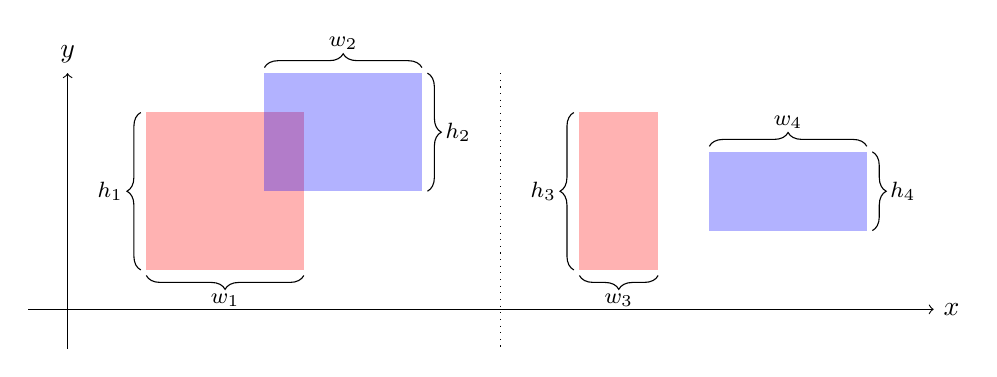
\begin{tikzpicture}[scale=1]

% Coordinates of Rectangle 1
\coordinate (A) at (1, .5);
\coordinate (B) at (3, .5);
\coordinate (C) at (3, 2.5);
\coordinate (D) at (1, 2.5);

% Coordinates of Rectangle 2
\coordinate (E) at (2.5, 1.5);
\coordinate (F) at (4.5, 1.5);
\coordinate (G) at (4.5, 3);
\coordinate (H) at (2.5, 3);

% Draw x/y axis
\draw[->] (-.5,0) -- (11,0) node[right] {\textbf{$x$}};
\draw[->] (0,-.5) -- (0,3) node[above] {\textbf{$y$}};
\draw[dotted] (5.5, 3) -- (5.5,-.5) node[above] {};

% Draw Rectangle 1 in transparent red
\fill[red, opacity=0.3] (A) -- (B) -- (C) -- (D) -- cycle;

% Draw Rectangle 2 in transparent blue
\fill[blue, opacity=0.3] (E) -- (F) -- (G) -- (H) -- cycle;

% Width labels for Rectangle 1
\draw[decorate, decoration={brace, amplitude=5pt, mirror, raise=2pt}] (A) -- (B) node[midway, below=5pt] {\footnotesize{}$w_1$};
\draw[decorate, decoration={brace, amplitude=5pt, raise=2pt}] (A) -- (D) node[midway, left=5pt] {\footnotesize{}$h_1$};

% Width labels for Rectangle 2
\draw[decorate, decoration={brace, amplitude=5pt, raise=2pt, mirror}] (G) -- (H) node[midway, above=5pt] {\footnotesize{}$w_2$};
\draw[decorate, decoration={brace, amplitude=5pt, raise=2pt, mirror}] (F) -- (G) node[midway, right=5pt] {\footnotesize{}$h_2$};

% Coordinates of Rectangle 3
\coordinate (I) at (6.5, .5);
\coordinate (J) at (7.5, .5);
\coordinate (K) at (7.5, 2.5);
\coordinate (L) at (6.5, 2.5);

% Coordinates of Rectangle 4
\coordinate (M) at (8.15, 1);
\coordinate (N) at (10.15, 1);
\coordinate (O) at (10.15, 2);
\coordinate (P) at (8.15, 2);

% Draw Rectangle 3 in transparent red
\fill[red, opacity=0.3] (I) -- (J) -- (K) -- (L) -- cycle;

% Draw Rectangle 4 in transparent blue
\fill[blue, opacity=0.3] (M) -- (N) -- (O) -- (P) -- cycle;

% Width labels for Rectangle 3
\draw[decorate, decoration={brace, amplitude=5pt, mirror, raise=2pt}] (I) -- (J) node[midway, below=5pt] {\footnotesize{}$w_3$};
\draw[decorate, decoration={brace, amplitude=5pt, raise=2pt}] (I) -- (L) node[midway, left=5pt] {\footnotesize{}$h_3$};

% Width labels for Rectangle 4
\draw[decorate, decoration={brace, amplitude=5pt, raise=2pt, mirror}] (O) -- (P) node[midway, above=5pt] {\footnotesize{}$w_4$};
\draw[decorate, decoration={brace, amplitude=5pt, raise=2pt, mirror}] (N) -- (O) node[midway, right=5pt] {\footnotesize{}$h_4$};
\end{tikzpicture}
\caption{Collision Detection Between Rectangles.}
\label{fig:collisiondetection}
\end{figure}

\begin{lstlisting}[language=MyJava]
abstract class GameObject {
  
  private int x;
  private int y;

  GameObject(int x, int y) {
    this.x = x;
    this.y = y;
  }
}
\end{lstlisting}


\begin{lstlisting}[language=Myjava]
abstract class AxisAlignedBoundingBoxObject extends GameObject {
  
  private int width;
  private int height;

  AxisAlignedBoundingBoxObject(int x, int y, int width, int height) {
    super(x, y);
    this.width = width;
    this.height = height;
  }

  /**
   * Determines whether this object collides with another AxisAlignedBoundingBoxObject.
   * @param obj - instance of AxisAlignedBoundingBoxObject.
   * @return true if the objects overlap and false otherwise.
   */
  boolean collidesWith(AxisAlignedBoundingBoxObject obj) {
    return (this.getX() < obj.getX() + obj.width) &&
	   (this.getX() + this.width >= obj.getX()) &&
 	   (this.getY() < obj.getY() + obj.height)  &&
	   (this.getY() + this.height >= obj.height); 
  }
}
\end{lstlisting}

We declared an abstract class to extend another abstract class; which is perfectly acceptable. Because it makes no sense to have an entity called \ttt{AxisAlignedBoundingBoxObject}, we declare it as abstract, but we need it to contain the functionality of \ttt{GameObject}, which calls for the inheritance. Normally, we would immediately write an extensive test suite for \ttt{collidesWith}, but because we cannot instantiate an \ttt{AxisAlignedBoundingBox} directly, we cannot test \ttt{collidesWith} at the moment. In a couple of paragraphs, however, this will be possible, with the additions of \ttt{CircleObject} and \ttt{RectangleObject}.

\begin{lstlisting}[language=MyJava]
import static Assertions.assertAll;
import static Assertions.assertEquals;

class AxisAlignedBoundingBoxObjectTester {

  @Test
  void testCollidesWith() {
    AxisAlignedBoundingBoxObject o1 = new RectangleObject(30, 30, 1000, 2000);
    AxisAlignedBoundingBoxObject o2 = new RectangleObject(0, 0, 5, 5);
    AxisAlignedBoundingBoxObject o3 = new RectangleObject(400, 200, 750, 250);
    AxisAlignedBoundingBoxObject o4 = new RectangleObject(300, 100, 300, 200);
    AxisAlignedBoundingBoxObject o5 = new CircleObject(20, 30, 1000);
    AxisAlignedBoundingBoxObject o6 = new CircleObject(200, 250, 500);
    AxisAlignedBoundingBoxObject o7 = new CircleObject(30, 300, 1500);
    AxisAlignedBoundingBoxObject o8 = new CircleObject(90, 85, 200);
    assertAll(
      () -> assertTrue(o1.collidesWith(o2)),
      () -> assertTrue(o1.collidesWith(o4)),
      () -> assertTrue(o2.collidesWith(o3)),
      () -> assertTrue(o2.collidesWith(o8)),
      () -> assertTrue(o3.collidesWith(o5)),
      () -> assertTrue(o5.collidesWith(o4)),
      () -> assertTrue(o6.collidesWith(o7)),
      () -> assertTrue(o7.collidesWith(o3)));
  }
}
\end{lstlisting}

We need to translate our circles into axis-aligned bounding box, but what does that mean? In short, we convert the given radius into the corresponding diameter, and designate this diameter as the width and height of the bounding box. Rectangular objects, on other hand, need no such fancy translation, since a bounding box is a rectangle. Neither subclasses storetheir dimensions as instance variables, due to the fact that the superclass takes care of this for us.

The question that we anticipate many readers are thinking of is, why do we even distinguish objects of differing ``types'' if they both implement collision detection in the same fashion? Since we are working in the context of a game, the way we draw these objects will almost certainly be different! Let's, for the sake of emphasizing the distinctions, design a \ttt{IDrawable} interface, which provides one method: \ttt{draw(Graphics2D g2d)}, which gives us a \ttt{Graphics2D} object. We will not discuss, nor do we really care about the innards of a graphics library aside from the fact that it contains two primitive methods: \ttt{drawOval(int x, int y, int w, int h)} and \ttt{drawRect(int x, int y, int w, int h)}. Therefore our two object subclasses will implement \ttt{IDrawable} and override the method differently.


\begin{lstlisting}[language=MyJava]
interface IDrawable {
  
  /**
   * Provides a means of drawing primitive graphics.
   * The inner details of "Graphics2D" are not important to us; 
   * we care about the fact that we can use the following methods:
   * 
   * - drawOval(int x, int y, int w, int h);
   * - drawRect(int x, int y, int w, int h);
   */
  void draw(Graphics2D g2d); 
}
\end{lstlisting} 

\begin{lstlisting}[language=MyJava]
class CircleObject extends AxisAlignedBoundingBoxObject implements IDrawable {
  
  CircleObject(int x, int y, int r) { super(x, y, r * 2, r * 2); }

  @Override
  void draw(Graphics2D g2d) {
    g2d.drawOval(this.getX(), this.getY(), this.getWidth(), this.getHeight());
  }
}
\end{lstlisting}

\begin{lstlisting}[language=MyJava]
class RectangleObject extends AxisAlignedBoundingBoxObject implements IDrawable {
  
  RectangleObject(int x, int y, int w, int h) { super(x, y, w, h); }
  
  @Override
  void draw(Graphics2D g2d) {
    g2d.drawRect(this.getX(), this.getY(), this.getWidth(), this.getHeight());
  }
}
\end{lstlisting}

\myexample{A terminal argument parser is a program/function that interprets a series of arguments passed to another program and makes it easier for programmers to determine if a flag is enabled. Without one, many programmers often resort to using a complex series of conditional statements to check for the existence of a flag. Not only is this cumbersome, but it is prone to errors, and neither extendable nor flexible to different arrangements of arguments. In this example we will develop a small terminal argument parser.}

First, we need to design a class that represents an ``argument'' to a program. Arguments, as we described in Chapter~\ref{chapter-arrays-collections}, are space-separated string values that we pass to a program executable, which populate the \ttt{String[] args} array in the \ttt{main} method. In particular, however, we want to specify that an argument is not necessarily the values themselves, but are instead the flags, or instructions, passed to the executable. The simplest version of a flag is one that receives exactly one argument, which we will represent via an abstract \ttt{Argument} class. Later on, we want to be able to validate a flag with its given arguments, so the \ttt{Argument} class includes an abstract \ttt{boolean validate} method, that shall be overridden in all subclasses of \ttt{Argument}.

\begin{lstlisting}[language=MyJava]
import java.util.List;
import java.util.Map;

abstract class Argument {

  private String key;

  Argument(String key) { this.key = key; }

  String getKey() { return this.key; }

  abstract boolean validate(Map<String, List<String>> args);
}
\end{lstlisting}

From here, let's design two types of arguments: one that is optional and one that receives $n$ arguments. Namely, an optional argument is one that is always valid, according to \ttt{validate}, because it does not necessarily need to exist. The $n$-valued argument, on the other hand, requires that the associated passed flag contains exactly $n$ values. For example, if we say that the \ttt{--input} flag requires exactly $3$ arguments, then if we do not pass exactly three space-separated non-flag values, it fails to validate.


\begin{lstlisting}[language=MyJava]
import java.util.List;
import java.util.Map;

class OptionalArgument extends Argument {

  OptionalArgument(String key) { super(key); }

  @Override
  boolean validate(Map<String, List<String>> args) { return true; }
}
\end{lstlisting}

\begin{lstlisting}[language=MyJava]
import java.util.List;
import java.util.Map;

class NumberedArgument extends Argument {

  private final int NUM_REQUIRED_ARGS;

  NumberedArgument(String key, int n) {
    super(key);
    this.NUM_REQUIRED_ARGS = n;
  }

  @Override
  boolean validate(Map<String, List<String>> args) {
    if (!args.containsKey(this.getKey())) { return false; } 
    else { return args.get(this.getKey()).size() == this.NUM_REQUIRED_ARGS; }
  }
}
\end{lstlisting}

Now comes the argument parser itself, which receives a string array of argument values, much like \ttt{main}, and extracts out the flags and arguments into a \ttt{Map<String, List<String$>$$>$} where the key represents the flag and the value is a list of the arguments to said flag. We also store a \ttt{Set<Argument>} to allow the programmer to designate arguments to the parser. The idea is straightforward: while traversing over \ttt{args}, if we encounter a string that begins with a double dash `\ttt{--}', it is qualified as a flag and the following arguments, up to another flag, are marked as arguments to the flag. We add these to the respective map as described before, and continue until we run out of elements in the array.

\begin{lstlisting}[language=MyJava]
import java.util.Map;
import java.util.HashMap;
import java.util.Set;
import java.util.HashSet;

class ArgumentParser {

  private Map<String, List<String>> parsedArguments;
  private Set<Argument> arguments;

  ArgumentParser(String[] args) {
    this.arguments = new HashSet<>();
    this.parsedArguments = new HashMap<>();
    String currKey = null;
    for (String arg : args) {
      if (arg.startsWith("--")) {
        currKey = arg.split("--")[1];
        this.parsedArguments.putIfAbsent(currKey, new ArrayList<>());
      } else if (currKey != null) {
        this.parsedArguments.get(currKey).add(arg);
      }
    }
  }

  void addArgument(Argument arg) { this.arguments.add(arg); }

  List<String> getArguments(String key) {
    return this.parsedArguments.containsKey(key) ? 
             this.parsedArguments.get(key) : 
             null;
  }
}
\end{lstlisting}

The \ttt{parseArguments} method returns whether or not the supplied arguments are valid according to the arguments populated via \ttt{addArgument}. Using streams, we verify that, after invoking \ttt{validate} on every argument, each separate call returns true, meaning that all arguments are valid and correct. Because it might be useful to return the associated arguments to a flag from a programmer's perspective who uses this parser, we include a \ttt{getArguments} method to return the list of arguments passed to a flag.

\begin{lstlisting}[language=MyJava]
import java.util.Map;
import java.util.HashMap;
import java.util.Set;
import java.util.HashSet;

class ArgumentParser {
  
  // ... other methods not shown.

  /**
   * Determines whether or not all of the arguments in the stored
   * instance variable are "valid".
   * @return true if all arguments are valid, false otherwise.
   */
  boolean parseArguments() {
    return this.arguments.stream()
                         .allMatch(e -> e.validate(this.parsedArguments));
  }
}
\end{lstlisting}

\subsubsection{The ASPL Interpreter}
\myexample{Inheritance is a truly powerful programming language construct, and we will now attempt to describe its beauty through the design of a mini-project. Said mini-project will encompass writing a small programming language called ASPL, or ``A Simple Programming Language.'' Programming language syntax and semantics, collectively, require a lot of knowledge outside the domain and scope of this text, but we will see that, even with our somewhat limited arsenal of tools, we can construct a fairly powerful programming language. Our language will start off as a recreation of the interpreter from our section on interfaces, but contains modifications to make it more flexible.}

As a means of motivation, let's write a few programs in this language to show its capabilities. The first listing is a simple program to add two numbers together. The second listing binds two variables, and if their sum is equal to 42, then the result is 100, otherwise it is zero. The third listing declares a variable, followed by a conditional, both cases of which contain another binding of a variable, closing off with a product operation.

\noindent % Prevents indentation at the beginning of the line
\begin{minipage}[t]{0.32\textwidth}
\begin{lstlisting}[language=MyScheme, frame=single]
(+ 25 17)
(*;\phantom{.};*)
(*;\phantom{.};*)
(*;\phantom{.};*)
(*;\phantom{.};*)
(*;\phantom{.};*)
(*;\phantom{.};*)
\end{lstlisting}
\end{minipage}%
\hfill % Fills the horizontal space between the minipages
\begin{minipage}[t]{0.32\textwidth}
\begin{lstlisting}[language=MyScheme, frame=single]
(let ([x 10])
  (let ([y 32])
    (if (eq? (+ x y) 42)
        100
        0)))

(*;\phantom{.};*)
\end{lstlisting}
\end{minipage}%
\hfill % Fills the horizontal space between the minipages
\begin{minipage}[t]{0.32\textwidth}
\begin{lstlisting}[language=MyScheme, frame=single]
(let ([z 42])
  (if (eq? (- 100 58) z)
      (let ([w -10])
        (* w z 2))
      (let ([w -5])
        (* z w -2))))
(*;\phantom{.};*)
\end{lstlisting}
\end{minipage}

Programming language syntax is often broken up into the nodes of an \emph{abstract syntax tree}, which at a quick glance is nothing more than a description of the operations of a language. To begin, we need to describe our programming language capabilities. To keep things simple, our language will contain integers, variables, a few arithmetic operators, and conditionals. It's important to note that, because we are glossing over the innards of lexing and  parsing, all of our tests will exist in the form of abstract syntax trees. We want an abstract AST node class from which every other AST node inherits. Then, we can design purpose-specific nodes that do what we wish. Every abstract syntax tree has a list of children node. We will also define a \texttt{toString} method that will print out the abstract syntax tree in a readable format. Our abstract syntax tree class uses two constructors: one that receives a list of abstract syntax tree nodes, and another that is variadic over the \ttt{AstNode} type. We implement two different constructors for convenience purposes during testing.

Additionally, we want our abstract syntax trees to be evaluable. Because ``evaluable'' describes a behavior of a class, we should throw this into an interface. We want its method, namely \ttt{eval}, to return something of type \ttt{AstNode} and receive an environment. For the time being, since we do not know what an \ttt{Environment} is, but we can still write the signature for the \ttt{eval} method. Notice, however, that we mark \ttt{eval} as \ttt{abstract} inside \ttt{AstNode}, because it is definitionally impossible to evaluate an \ttt{AstNode}, since evaluation behavior is dependent on the subclasses and how they interact.

\begin{lstlisting}[language=MyJava]
import java.util.List;

abstract class AstNode {

  private final List<AstNode> CHILDREN;  
 
  AstNode(List<AstNode> children) { 
    this.CHILDREN = children; 
  }

  AstNode(AstNode... children) { 
    this(List.of(children)); 
  }

  abstract AstNode eval(Environment env);

  List<AstNode> getChildren() { 
    return this.CHILDREN; 
  }

  public abstract String toString();
}
\end{lstlisting}

From here, the simplest three abstract syntax tree nodes are \ttt{VarNode}, \ttt{NumNode}, and \ttt{BoolNode}, corresponding to variables, numbers, and booleans, respectively. Each of these nodes will have a single value, that being the variable name, number, or boolean. The \ttt{eval} methods of the latter two classes resolve to themselves, since evaluating a number or a boolean is itself. The former, that being \ttt{VarNode}, is a little trickier. 

We must consider what happens when we evaluate a variable in any other programming language. The language looks up the variable identifier in the list of accessible bindings and returns whatever is the corresponding value. This location of bindings is called an environment in the programming languages nomenclature, and generally takes the form of a \ttt{HashMap} data structure. Therefore we can store an instance of a \ttt{HashMap} in our \ttt{Environment} class. 

As a final corollary point before jumping into the environment details, we must override \ttt{.equals} and \ttt{.hashCode} in these three atomic value classes. In theory, we could override them in the other classes as well. For the time being, because our programs always resolve to one of these three types (and because our test cases only operate over the three), we will only override the definitions in these classes.

The question now is of what type are the keys and values in our map. The keys are string identifiers, and the values are their corresponding abstract syntax trees. Our environment representation/class is extremely simple and almost seems superfluous, but in due time we will add more functionality to justify its existence over a simple \ttt{HashMap} instance. In particular, the \ttt{lookup} method for finding a variable association will remain undefined for now.

\begin{lstlisting}[language=MyJava]
import java.util.HashMap;
import java.util.Map;

final class Environment {
  
  private final Map<String, AstNode> ENV;

  Environment() { 
    this.ENV = new HashMap<>(); 
  }

  AstNode lookup(String var) { /* TODO. */ }
}
\end{lstlisting}

\begin{lstlisting}[language=MyJava]
import static Assertions.assertEquals;
import static Assertions.assertAll;

class AstTest {

  @Test
  void testVarNode() {
    assertEquals("x", new VarNode("x").toString());
  }

  @Test
  void testNumNode() {
    assertEquals("42", new NumNode("42").toString());
  }

  @Test
  void testBoolNode() {
    assertEquals("true", new BoolNode("true").toString());
    assertEquals("false", new BoolNode("false").toString());
  }  
}
\end{lstlisting}


\begin{lstlisting}[language=MyJava]
final class VarNode extends AstNode {

  private final String NAME;

  VarNode(String name) {
    super();
    this.NAME = name;
  }

  /**
   * Interpret a variable. We look up the variable in the environment and
   * return the value associated with it.
   * @param env - the environment in which to interpret the variable.
   * @return The result of the variable lookup after interpretation.
   */
  @Override
  AstNode eval(Environment env) {
    String id = this.NAME;
    AstNode res = env.lookup(id);
    return res.eval(env);
  }

  @Override
  public String toString() { 
    return this.NAME; 
  }
}
\end{lstlisting}

\begin{lstlisting}[language=MyJava]
final class NumNode extends AstNode {

  private final double VALUE;

  NumNode(String value) {
    super();
    this.VALUE = Double.parseDouble(value);
  }

  NumNode(double value) { 
    this(Double.toString(value)); 
  }

  @Override
  AstNode eval(Environment env) { 
    return this;
  }

  @Override
  public boolean equals(Object o) {
    if (!(o instanceof NumNode)) { return false; }
    else { return this.VALUE == ((NumNode) o).VALUE; }
  }

  @Override
  public int hashCode() {
    return Objects.hash(this.VALUE);
  }

  @Override
  public String toString() { 
    return Double.toString(this.VALUE); 
  }

  public double getValue() {
    return this.VALUE;
  }
}
\end{lstlisting}


\begin{lstlisting}[language=MyJava]
final class BoolNode extends AstNode {

  private final boolean VALUE;

  BoolNode(String value) {
    super();
    this.VALUE = Boolean.parseBoolean(value);
  }

  BoolNode(boolean value) { 
    this(Boolean.toString(value)); 
  }

  @Override
  AstNode eval(Environment env) { 
    return this; 
  }

  @Override
  public boolean equals(Object o) {
    if (!(o instanceof BoolNode)) { return false; }
    else { return this.VALUE == ((BoolNode) o).VALUE; }
  }
  
  @Override
  public int hashCode() {
    return Objects.hashCode(this.VALUE);
  }

  @Override
  public String toString() { 
    return Boolean.toString(this.VALUE); 
  }

  public boolean getValue() {
    return this.VALUE;
  }
}
\end{lstlisting}

From here, we arrive at primitive operators via \ttt{PrimNode}. A primitive operator is one akin to addition, subtraction, and so forth. Two additional primitives that we will support are reading an integer from standard input, and printing one to standard output. Primitive operators receive any number of arguments and whose behavior is handled as a case analysis of the \ttt{eval} method. 


\begin{lstlisting}[language=MyJava]
import java.util.List;

final class PrimNode extends AstNode {

  private final String OP;

  PrimNode(String op, AstNode... children) {
    super(children);
    this.OP = op;
  }

  /**
   * Interpret a primitive operation.
   * @param env - the environment in which to interpret the operation.
   * @return The result of the primitive operation.
   */
  @Override
  AstNode eval(Environment env) {
    String op = this.OP;
    List<AstNode> operands = this.getChildren().stream()
            .map(n -> n.eval(env))
            .toList();
    switch (op) {
      case "+": return this.primPlus(operands, env);
      case "-": return this.primMinus(operands, env);
      case "*": return this.primProduct(operands, env);
      case "eq?": return this.primEq(operands, env);
      default: return null;
    }
  }

  @Override
  public String toString() {
    return String.format("(%s %s)", this.OP, this.getChildren().toString());
  }

  private AstNode primPlus(List<AstNode> args, Environment env) {
    return new NumNode(args.stream()
                              .map(t -> ((NumNode) t).getValue())
                              .reduce(0.0, Double::sum));
  }

  private AstNode primMinus(List<AstNode> args, Environment env) {
    double res = ((NumNode) args.get(0)).getValue();
    for (int i = 1; i < args.size(); i++) {
      res -= ((NumNode) args.get(i)).getValue();
    }
    return new NumNode(res);
  }

  private AstNode primProduct(List<AstNode> args, Environment env) {
    return new NumNode(args.stream()
                              .map(t -> ((NumNode) t).getValue())
                              .reduce(1.0, (a, c) -> c * a)));
  }

  private AstNode primEq(List<AstNode> args, Environment env) {
    return new BoolNode(args.get(0).equals(args.get(1)));
  }
}
\end{lstlisting}

We need a way of binding variables to their values, so we shall take a hint from functional programming languages via the \ttt{LetNode} class. The \ttt{LetNode} class has three children: a variable name, a value, and a body. The variable name will be a string, with the value and body both being abstract syntax tree nodes. The \ttt{LetNode} class will have a \ttt{toString} method that will return a string in the form of \ttt{(let ([<var> <exp>]) <body>)}. The \ttt{eval} method will evaluate the value, extend the environment with the new binding, and then evaluate the body with the extended environment. To do this, we need to understand what environment extension entails. Reconsidering our \ttt{Environment} class, we know that it contains a \ttt{HashMap} to designate that environments use maps by design. We may be tempted to write a \ttt{set} method in our \ttt{Environment} class to add an identifier binding to the current environment. Although this works (and will be a necessity in due time), it means that we can only \emph{modify}, or \emph{change}, the environment, which isn't desired. The alternative approach would be to utilize \emph{environment extension}. That is, create a new environment with the old bindings, followed by an insertion of the new binding. Environment extension brings up the issue of variable scope, because different variables are live at different locations in the program. Consider the following program described by the abstract syntax tree:

\begin{verbnobox}[\small]
new LetNode("x", new NumNode(5), 
 new LetNode("y", new PrimNode("+", new NumNode(6), new VarNode("x")), 
  new VarNode("y")))
\end{verbnobox}
  
Within the inner-most \ttt{PrimNode} expression, $x$ does not exist in its environment, but it does exist in an environment defined above its scope. So, each environment is itself a store a map of identifiers to abstract syntax trees, but they also contain another \ttt{Environment}. If we are at the ``root level'' of the program, this environment is set to \ttt{null}. Correspondingly, Environment contains two constructors: one that receives a parent environment and another without. As such, we must write the \ttt{lookup} method, which finds a variable binding in the current list of bindings and, if it does not exist, recursively looks it up in the parent environment. If we reach the root level environment and the variable does not exist, we return a \ttt{null} value. We also override the \ttt{toString} method to print out the environment in a readable format.

\begin{lstlisting}[language=MyJava]
import static Assertions.assertEquals;
import static Assertions.assertAll;

class EnvironmentTester {
  
  @Test
  void testEnvironment() {
    Environment root = new Environment();
    Environment e1 = env.extend("x", new NumNode(5));
    Environment e2 = env.extend("y", new NumNode(6));
    assertAll(
      () -> assertEquals(new NumNode(5), env.lookup("x")),
      () -> assertEquals(new NumNode(6), env.lookup("y")),
      () -> assertEquals(null, env.lookup("z")),
      () -> assertEquals(null, env.lookup("x")));
  }
}
\end{lstlisting}
  

\begin{lstlisting}[language=MyJava]
import java.util.HashMap;
import java.util.Map;

final class Environment {

  private final Map<String, AstNode> ENV;
  private final Environment PARENT;

  Environment() { 
    this(null); 
  }

  Environment(Environment parent) { 
    this.ENV = new HashMap<>(); 
    this.PARENT = parent; 
  }

  /**
   * Looks up a variable in the current environment.
   * @param id - the variable name.
   * @return the value bound to the variable, or null if it does not exist.
   */
  AstNode lookup(String id) {
    if (this.ENV.containsKey(id)) { return this.ENV.get(id); } 
    else if (this.PARENT != null) { return this.PARENT.lookup(id); } 
    else { return null; }
  }

  /**
   * Extends the current environment to contain a new variable binding.
   * @param id - the variable name.
   * @param value - the value to bind to the variable.
   * @return a new environment with the new binding.
   */
  Environment extend(String id, AstNode value) {
    Environment env = new Environment(this);
    env.ENV.put(id, value);
    return env;
  }
}
\end{lstlisting} 

Our modified version of the environment allows us to implement local/let bindings in a way that respects parent environments. As one of the exercises of this chapter demonstrate, environment extension helps us when adding user-defined functions.

\begin{lstlisting}[language=MyJava]
final class LetNode extends AstNode {

  private final String ID;

  LetNode(String id, AstNode exp, AstNode body) {
    super(exp, body);
    this.ID = id;
  }

  /**
   * Interpret a let statement. A new environment is introduced 
   * in which the let body is evaluated.
   * @param env - The environment in which to interpret the let binding.
   * @return The result of the let statement.
   */
  @Override
  AstNode eval(Environment env) {
    String id = this.ID;
    AstNode exp = this.getChildren().get(0);
    AstNode body = this.getChildren().get(1);

    // Interpret the expression and convert it into its AST.
    AstNode newExp = exp.eval(env);
    Environment e1 = env.extend(id, newExp);
    return body.eval(e1);
  }

  @Override
  public String toString() {
    AstNode e = this.getChildren().get(0);
    AstNode b = this.getChildren().get(1);
    return String.format("(let ([%s %s]) %s)", this.ID, e.toString(), b.toString());
  }
}
\end{lstlisting}

Finally we arrive at decision-based nodes. The \ttt{IfNode} class represents a conditional expression rather than a statement. Recall the ternary operator; it resolves to a value, unlike Java's \ttt{if} statement. The \ttt{IfNode} class has three children: a predicate, a consequent, and an alternative. The predicate is an abstract syntax tree that represents a boolean expression, and the consequent and alternative are arbitrary abstract syntax tree nodes. The \ttt{IfNode} class will have a \ttt{toString} method that will return a string of the form \ttt{(if <pred> <conseq> <alt>)}. Its evaluator will evaluate the predicate, and then evaluate either the consequent or alternative depending on the result of the predicate.


\begin{lstlisting}[language=MyJava]
final class IfNode extends AstNode {
  
  IfNode(AstNode predicate, AstNode consequent, AstNode alternative) {
    super(predicate, consequent, alternative);
  }

  /**
  * Interpret an if statement.
  * @param env - the environment in which to interpret the if statement.
  * @return The result of the if statement.
  */
  @Override
  AstNode eval(Environment env) {
    AstNode pred = this.getChildren().get(0);
    AstNode cons = this.getChildren().get(1);
    AstNode alt = this.getChildren().get(2);

    // Evaluate the predicate, then interpret one way or the other.
    if (pred.eval(env).getBooleanValue()) { return cons.eval(env); } 
    else { return alt.eval(env); }
  }
  
  @Override
  public String toString() {
    AstNode p = this.getChildren().get(0);
    AstNode c = this.getChildren().get(1);
    AstNode a = this.getChildren().get(2);
    return String.format("(if %s %s %s)", p.toString(), c.toString(), a.toString());
  }
}
\end{lstlisting}

Finally, at long last, we can write some tests! We will store each test in a class called \ttt{InterpTester}, which polymorphically tests the evaluation method of the abstract syntax tree methods. These tests all receive a blank environment representing the global environment, which contains no bindings at the start of evaluation. Unfortunately, we still have to write the programs as an abstract syntax tree, but the problems of lexing and parsing raw string input into an abstract syntax tree are reserved for some other time (or perhaps a separate course altogether).


\begin{lstlisting}[language=MyJava]
import static Assertions.assertAll;
import static Assertions.assertEquals;
  
class InterpTester {
  
  @Test
  void testEval() {
    assertAll(
      () -> assertEquals(new NumNode("42"),
                         new NumNode("42").eval(new Environment())),
      () -> assertEquals(new BoolNode(true),
                         new PrimNode("eq?",
                          new NumNode(42),
                          new PrimNode("-",
                           new NumNode(100),
                           new NumNode(58))).eval(new Environment())),
      () -> assertEquals(new NumNode("42"),
                         new LetNode("x", 
                          new NumNode("42"), 
                          new VarNode("x")).eval(new Environment())),
      () -> assertEquals(new NumNode("42"),
                         new LetNode("x", new NumNode("1"),
                          new LetNode("y", new NumNode("41"),
                           new PrimNode("+", 
                            new VarNode("x"), 
                            new VarNode("y")))).eval(new Environment())));
  }
}
\end{lstlisting}

In general, object-oriented programs with inheritance should be structured as a sequence of specific subclasses that extend an abstract class, as we have done with the different abstract syntax tree node types and the root \ttt{AstNode} abstract class. 


\newpage
\section{Exercises}

\myexercise{1}{chapter-classes}{This exercise has 3 parts.}

The \emph{Kotlin} programming language supports customized \emph{ranges}. That is, we can define an interval using dot notation, e.g., \ttt{1..10}, then query a value over that interval. For instance, \ttt{x in 1..10} returns whether or not \ttt{x} is between \ttt{1} and \ttt{10}, inclusive. This comparison, however, extends beyond primitive datatypes; ranges may operate over classes. For example, we can create a range \ttt{"hi".."howdy"}, which defines the range of strings in between \ttt{"hi"} and \ttt{"howdy"}.

\begin{enumerate}[label=(\alph*)]
    \item Design the generic \ttt{Range} class. It should store, as instance variables, a minimum and a maximum value, both of which are of type \ttt{<T extends Comparable<T>>}, meaning \ttt{T} must be a comparable type.
    \item The \ttt{Range} constructor should receive these two values as parameters and assign them to the instance variables accordingly. 
    \item Design the \ttt{boolean contains(T v)} method that returns whether or not $v$ is between the interval that this range operates over. 
\end{enumerate}

\myexercise{2}{chapter-advanced-oop}{Design the generic static method \ttt{T validateInput(String prompt, String errResp, U extends Predicate<T> p)} that receives a prompt, an error response, and an object that implements the \ttt{Predicate} interface to test whether or not the received value, received through standard input, is valid. If the value is invalid according to the predicate, print the error response and re-prompt the user. Otherwise, return the entered value.}

\myexercise{3}{chapter-advanced-oop}{A \emph{lazy list} is one that, in theory, produces infinite results! Consider the \ttt{ILazyList} interface below:}
\begin{lstlisting}[language=MyJava]
interface ILazyList<T> {
  T next();
}
\end{lstlisting}

When calling \ttt{next} on a lazy list, we update the contents of the lazy list and return the next result. We mark this as a generic interface to allow for any desired return type. For instance, below is a lazy list that produces factorial values:\footnote{We will ignore the intricacies that come with Java's implementation of the \ttt{int} datatype. To make this truly infinite, we could use \ttt{BigInteger}.}
\begin{lstlisting}[language=MyJava]
class FactorialLazyList implements ILazyList<Integer> {

  private int n;
  private int fact;
 
  FactorialLazyList() {
    this.n = 1;
    this.fact = 1;
  }

  @Override
  int next() {
    this.fact *= this.n;
    this.n++;
    return this.fact;
  }
}
\end{lstlisting}

Testing it with ten calls to \ttt{next} yields predictable results.

\begin{lstlisting}[language=MyJava]
import static Assertions.assertAll;
import static Assertions.assertEquals;

class FactorialLazyListTester {

  @Test
  void testFactorialLazyList() {
    ILazyList<Integer> FS = new FactorialLazyList();
    assertAll(
      () -> assertEquals(1, FS.next()),
      () -> assertEquals(2, FS.next()),
      () -> assertEquals(6, FS.next()),
      () -> assertEquals(24, FS.next()),
      () -> assertEquals(120, FS.next()),
      () -> assertEquals(720, FS.next()),
      () -> assertEquals(5040, FS.next()),
      () -> assertEquals(40320, FS.next()),
      () -> assertEquals(362880, FS.next()),
      () -> assertEquals(3628800, FS.next()));
  }
}
\end{lstlisting}

Design the \ttt{FibonacciLazyList} class, which implements \ttt{ILazyList<Integer>} and correctly overrides \ttt{next} to produce Fibonacci sequence values. You code should \emph{not} use any loops or recursion. Recall that the Fibonacci sequence is defined as $f(n) = f(n - 1) + f(n - 2)$ for all $n\geq{2}$. The base cases are $f(0) = 0$ and $f(1) = 1$.

\begin{lstlisting}[language=MyJava]
import static Assertions.assertAll;
import static Assertions.assertEquals;

class FibonacciLazyListTester {

  @Test
  void testFibonacciLazyList() {
    ILazyList<Integer> FS = new FibonacciLazyList();
    assertAll(
      () -> assertEquals(0, FS.next()),
      () -> assertEquals(1, FS.next()),
      () -> assertEquals(1, FS.next()),
      () -> assertEquals(2, FS.next()),
      () -> assertEquals(3, FS.next()),
      () -> assertEquals(5, FS.next()),
      () -> assertEquals(8, FS.next()),
      () -> assertEquals(13, FS.next()),
      () -> assertEquals(21, FS.next()),
      () -> assertEquals(34, FS.next()));
  }
}
\end{lstlisting}

\myexercise{2}{chapter-advanced-oop}{Design the \ttt{LazyListTake} class. It should receive an \ttt{ILazyList} and an integer $n$ denoting how many elements to take, as parameters. Then, write a \ttt{List<T> getList()} method, which returns a \ttt{List<T>} of $n$ elements from the given lazy list.}


\begin{lstlisting}[language=MyJava]
import static Assertions.assertAll;
import static Assertions.assertEquals;

class LazyListTakeTester {

 @Test
 void testLazyListTake() {
  LazyListTake llt1 = new LazyListTake(new FactorialLazyList(), 10);
  LazyListTake llt2 = new LazyListTake(new FibonacciLazyList(), 10);

  assertAll(
    () -> assertEquals("[1, 2, 6, 24, 120, 720, 5040, 40320, 362880, 3628800]",
                       llt1.getList().toString()),
    () -> assertEquals("[0, 1, 1, 2, 3, 5, 8, 13, 21, 34]",
                       llt2.getList().toString()));
 }
}
\end{lstlisting}

\myexercise{2}{chapter-advanced-oop}{Java's functional API allows us to pass lambda expressions as arguments to other methods, as well as method references (as we saw in Chapter~\ref{chapter-arrays-collections}). Design the generic \ttt{FunctionalLazyList} class to implement \ttt{ILazyList}, whose constructor receives a unary function \ttt{Function<T, T> f} and an initial value \ttt{T t}. Then, override the \ttt{next} method to invoke $f$ on the current element of the lazy list and return the previous. For example, the following test case shows the expected results when creating a lazy list of infinite positive multiples of three.}

\begin{lstlisting}[language=MyJava]
import static Assertions.assertEquals;
import static Assertions.assertAll;

class FunctionalLazyListTester {

  @Test
  void testMultiplesOfThreeLazyList() {
    ILazyList<Integer> mtll = new FunctionalLazyList<>(x -> x + 3, 0);
    assertAll(
      () -> assertEquals(0, mtll.next()),
      () -> assertEquals(3, mtll.next()),
      () -> assertEquals(6, mtll.next()),
      () -> assertEquals(9, mtll.next()),
      () -> assertEquals(12, mtll.next()));
  }
}
\end{lstlisting}

What's awesome about this exercise is that it allows us to define the elements of the lazy list as any arbitrary lambda expression, meaning that we could redefine \ttt{FactorialLazyList} and \ttt{FibonacciLazyList} in terms of \ttt{FunctionLazyList}. We can generate infinitely many ones, squares, triples, or whatever else we desire.

\myexercise{2}{chapter-advanced-oop}{Design the generic \ttt{CyclicLazyList} class, which implements \ttt{ILazyList}, whose constructor is variadic and receives any number of values. Upon calling \ttt{next}, the cyclic lazy list should return the first item received from the constructor, then the second, and so forth until reaching the end. After returning all the values, cycle back to the front and continue. For instance, if we invoke \ttt{new CyclicLazyList<Integer>(1, 2, 3)}, invoking \ttt{.next} five times will produce \ttt{1}, \ttt{2}, \ttt{3}, \ttt{1}, \ttt{2}.}

\myexercise{1}{chapter-advanced-oop}{Design the \ttt{static <T> Predicate<T> orEquals(Predicate<T> pred, T x)} method that, when given a predicate $p$ and an object $x$, returns a \emph{new} predicate that returns true if its argument $x'$ is equal (using \ttt{.equals}) to $x$ or satisfies $p(x)$.}

\myexercise{2}{chapter-advanced-oop}{Design the \ttt{static <T> List<T> predicateOrEquals(List<T> ls, Predicate<T> pred, BiFunction<T, T, Boolean>, T x)} method that, when given a list of values $ls$, a predicate $p$, a function $f$, and a value $x$ that returns the list of values in $ls$ that either satisfy $p$ or are equal according to $f$. For the purposes of this question, $f$ is a method of two arguments of type $T$ that determines whether or not they are ``equal'' according to some criteria.}

\myexercise{1}{chapter-advanced-oop}{Design the \ttt{static <T> boolean andMap(List<T> ls, Predicate<T> pred)} method that returns whether or not all elements of the input list satisfy the given predicate. Use the stream API to solve this problem, but do \emph{not} use the \ttt{allMatch} method, as that method solves the problem we want \emph{you} to solve!}

\myexercise{2}{chapter-advanced-oop}{Design the \ttt{static <T, U> U foldr(List<T> ls, BiFunction<T, U, U> f, U u)} method that receives a list of values $ls$, a function $f$, and an initial value $u$. The method should return the result of folding the list from the right with the given function and initial value. By ``folding,'' we mean that we apply $f$ to the last element of the list and the initial value, then apply $f$ to the second-to-last element and the result of the previous application, and so forth. To think of this in terms of infix notation over some list, consider the list $[a, b, c, d]$. Folding it over the function $\circ$ and initial value $u$ is $a \circ (b \circ (c \circ (d \circ u)))$. Do \emph{not} use the \ttt{reduce} method, as that method solves the problem we want \emph{you} to solve!}

\myexercise{1}{chapter-advanced-oop}{Design the \ttt{static <T, U> List<U> buildList(int n, Function<T, U> f)} method that receives an integer $n$ and a function $f$ and returns a list of $n$ elements, where the $i^\text{th}$ element is $f(i)$. For example, if we invoke \ttt{buildList(5, x -> x * x)}, we should receive the list $[1, 4, 9, 16, 25]$.}

\myexercise{1}{chapter-advanced-oop}{This exercise involves the doubly-linked list we wrote in the chapter.}
Design the \ttt{int size()} method, which returns the number of elements in the list. You can do this either recursively or with a loop. For better practice, try (and thoroughly test) both implementations.

\myexercise{2}{chapter-advanced-oop}{This exercise involves the doubly-linked list we wrote in the chapter.}
Design the \ttt{void set(int i, T v)} method, which overwrites/assigns, at index $i$, the value $v$. If the provided index is out-of-bounds, do nothing.

\myexercise{2}{chapter-advanced-oop}{This exercise involves the doubly-linked list we wrote in the chapter.}
Design the \ttt{void insert(int i, T v)} method, which inserts the value $v$ at index $i$. As an example, if we insert $4$ into the list $[20, 5, 100, 25]$ at index $2$, the list then becomes $[20, 5, 4, 100, 25]$. If the provided index is out-of-bounds, do nothing.

\myexercise{1}{chapter-advanced-oop}{This exercise involves the interpreter we wrote in the chapter.}
Add the \ttt{"read-number"} and \ttt{"print"} primitive operations to the language. The latter is polymorphic, meaning it can print both numbers and booleans.

\myexercise{2}{chapter-advanced-oop}{This exercise involves the interpreter we wrote in the chapter.}
Functional programming languages, in general, are a composition of expressions, wherein statements are more of an afterthought. To this end, design the \ttt{BeginNode} abstract syntax tree node, which receives a list of abstract syntax trees. At the interpreter level, the \ttt{BeginNode} should evaluate each of the abstract syntax trees in the list, and return the result of the last one.

\myexercise{2}{chapter-advanced-oop}{This exercise involves the interpreter we wrote in the chapter.}
Variables, in our language, are defined and bound exactly once, namely when they are defined within a let node. Though, in imperative programming, it is often crucial to allow variable reassignments. Design the \ttt{SetNode} class, which receives a variable and an abstract syntax tree, and reassigns the variable to the result of the abstract syntax tree. At the interpreter level, the \ttt{SetNode} should evaluate the abstract syntax tree, and reassign the variable to the result in the current environment (and only the current environment). This means that you'll need to modify the \ttt{Environment} class to allow for variable reassignments. Hint: create a \ttt{set} method in the \ttt{Environment} class.

\myexercise{2}{chapter-advanced-oop}{This exercise involves the interpreter we wrote in the chapter.} Recursion is nice and intuitive, for the most part. Unfortunately, it is not always the most efficient way to solve a problem. For example, the Fibonacci sequence, as we saw in Chapter~\ref{chapter-crl}, is often defined recursively, but it is much more efficient to define it iteratively (or even with tail recursion). Design the \ttt{WhileNode} class, which receives a condition and an abstract syntax tree, and evaluates the abstract syntax tree until the condition is false. At the interpreter level, the \ttt{WhileNode} should evaluate the condition, and if it is true, evaluate the abstract syntax tree, and repeat until the condition is false. To test your implementation, you will need to combine the \ttt{WhileNode} with both the \ttt{SetNode} and \ttt{BeginNode} classes.

\myexercise{3}{chapter-advanced-oop}{This exercise involves the interpreter we wrote in the chapter.} Having to manually update our case analysis on the primitive operator type is cumbersome and prone to mistakes. A better solution would be to store the operator and its corresponding ``handler'' method, i.e., the method that receives the operands and does the logic of the operator. We can do this via a map where the keys are the string operators and the values are functional references to the handlers. Unfortunately, Java does not directly support passing methods as parameters, meaning they are not first-class. Conversely, we can make use of Java's functional interfaces to achieve our goal. Namely, the interface will contain one method: \ttt{AstNode apply(List<AstNode> args, Environment env)}, where \ttt{args} is the list of evaluated arguments. We will call the interface \ttt{IFunction} and make it generic, with the first type quantified to a list of \ttt{AstNode} instances, and the second type quantified to \ttt{AstNode}. Hopefully, the connection between these quantified types and the signature of \ttt{apply} is apparent. Using the below definition of \ttt{IFunction}, update \ttt{PrimNode} to no longer perform a case analysis in favor of the map. We provide an example of populating the map with the initial operators in a \ttt{static} block.

\begin{lstlisting}[language=MyJava]
@FunctionalInterface
interface IFunction<T, R> {
  
  R apply(T t);
}
\end{lstlisting}


\begin{lstlisting}[language=MyJava]
import java.util.Map;
import java.util.HashMap;

class PrimNode extends AstNode {
  
  private static final Map<String, IFunction<List<AstNode>, AstNode>> OPERATORS;
  
  static {
    OPERATORS = new HashMap<>();
    OPERATORS.put("+", this.primPlus);
  }

  @Override
  AstNode eval(Environment env) { /* TODO. */  }

  private AstNode primPlus(List<AstNode> args, Environment env) { /* Details omitted. */ }
}
\end{lstlisting}

\myexercise{3}{chapter-advanced-oop}{This exercise is multi-part and involves the interpreter we wrote in the chapter.}
\begin{enumerate}[label=(\alph*)]
  \item First, design the \ttt{ProgramNode} class, which allows the user to define a program as a sequence of statements rather than a single expression.
  \item Design the \ttt{DefNode} class, which allows the user to create a global definition. Because we're now working with definitions that do not extend the environment, we should use the set method in environment. When creating a global definition via \ttt{DefNode}, we're expressing the idea that, from that point forward, the (root) environment should contain a binding from the identifier to whatever value it binds.
  \item Design the \ttt{FuncNode} node. We will consider a function definition as an abstract tree node that begins with \ttt{FuncNode}. This node has two parameters to its constructor: a list of parameter (string) identifiers, and a single abstract syntax tree node representing the body of the function. We will only consider functions that return values; void functions do not exist in this language.
  \item Design the \ttt{ApplyNode} class, which applies a function to its arguments. You do not need to consider applications in which the first argument is a non-function. 

  Calling/Invoking a function is perhaps the hardest part of this exercise. Here's the idea, which is synonymous and shared with almost all programming languages: 

  \begin{enumerate}[label=(\roman*)] 
  \item First, evaluate each argument of the function call. This will result in several evaluated abstract syntax trees, which should be stored in a list. 
  \item We then want to create an environment in which the formal parameters are bound to their arguments. Overload the extend method in \ttt{Environment} to now receive a list of string identifiers and a list of (evaluated) AST arguments. Bind each formal to its corresponding AST, and return the extended environment. 
  \item Evaluate the function identifier to get its function definition as an abstract syntax tree.
  \item Call \ttt{eval} on the function body and pass the new (extended) environment.
  \end{enumerate}
  This seems like a lot of work (because it is), but it means you can write really cool programs, including those that use recursion!
  \begin{verbnobox}[\small]
new ProgramNode(
  new DefNode("!", 
    new FuncNode(
      List.of("n"),
      new IfNode(
        new PrimNode("eq?", 
          new VarNode("n"), 
          new NumNode(0)),
        new NumNode(1),
        new PrimNode("*", 
          new VarNode("n"), 
          new ApplyNode("!", 
            new PrimNode("-", 
            new VarNode("n"), 
            new NumNode(1))))))),
  new PrimNode("print", new ApplyNode("!", new NumNode(5)))
)
\end{verbnobox}
\end{enumerate}

\myexercise{3}{chapter-advanced-oop}{This exercise involves the interpreter we wrote in the chapter.}
Data structures are a core and fundamental feature of programming languages. A language without them, or at least one to build others on top of, suffers severely in terms of usability. We will implement a \emph{cons}-like data structure for our interpreter. In functional programming, we often use three operations to act on data structures akin to linked lists: \emph{cons}, \emph{first}, and \emph{rest}, to construct a new list, retrieve the first element, and retrieve the rest of the list respectively. We can inductively define a cons list as follows:

\begin{verbnobox}[\small]
A ConsList is one of:
 - new ConsList()
 - new ConsList(x, ConsList)
\end{verbnobox}

Implement the cons data structure into your interpreter. This should involve designing the \ttt{ConsNode} class that conforms to the aforementioned data definition. Moreover, you will need to update \ttt{PrimNode} to account for the \ttt{first} and \ttt{rest} primitive operations, as well as an \ttt{empty?} predicate, which returns whether or not the cons list is empty. Finally, update the \ttt{AstNode} class to print a stringified representation of a \ttt{ConsNode}, which amounts to printing each element, separated by spaces, inside of brackets, e.g., \ttt{[$l_0, l_1, ..., l_{n-1}]$}.

\myexercise{2}{chapter-advanced-oop}{This exercise involves the interpreter we wrote in the chapter.}
Having to manually type out the abstract syntax tree constructors when writing tests is extremely tedious. Design a \emph{lexer} for the language described by the interpreter. That is, the text is broken up into tokens that are then categorized. For example, \ttt{'('} might become \ttt{OPEN\_PAREN}, \ttt{"lambda"} might become \ttt{SYMBOL}, \ttt{"variable-name"} might become \ttt{SYMBOL}, and \ttt{123.45} might become \ttt{NUMBER}. The output of the lexer is a list of tokens. Part of the trick is to ensure that after reading an open parenthesis, the next token is not grabbed as part of the open parenthesis.

\myexercise{3}{chapter-advanced-oop}{This exercise involves the interpreter we wrote in the chapter.}
Design a parser for the language described by the interpreter. The idea is to tokenize a raw string, then parse the tokens to create an abstract syntax tree that represents the program. A good starting point would be to parse \emph{all} parenthesized expressions into what we will call \ttt{SExprNode}, then traverse over the tree to ``correct'' them into their true nodes, e.g., whether they are \ttt{IfNode}, \ttt{LetNode}, and so forth. Realistically, all programs in our language are, at their core, either primitive values or s-expressions.

\myexercise{2}{chapter-advanced-oop}{This exercise involves the interpreter we wrote in the chapter.}
The Scheme programming language and its derivatives support \emph{code quotation}, i.e., the ability to convert an evaluable expression into data. As an example, if we evaluate \ttt{new QuoteNode(new VarNode("x"))}, we receive a symbol as the output, rather than the evaluated symbol via environment lookup. Add the \ttt{QuoteNode} class to your interpreter.

\myexercise{3}{chapter-advanced-oop}{In Chapter~\ref{chapter-crl}, we discussed tail recursion and an action performed by some programming languages known as tail-call optimization. We know that we can convert any (tail) recursive algorithm into one that uses a loop, and we described said process in the chapter. There is yet another approach that we can mimic in Java with a bit of trickery and interfaces.}

The problem with tail recursion (and recursion in general) in Java is the fact that it does not convert tail calls into iteration, which means the stack quickly overflows with activation records. We can make use of a \emph{trampoline} to force the recursion into iteration through \emph{thunks}. In essence, we have a tail recursive method that returns either a value or makes a tail recursive call, such as the factorial example below.\footnote{We omit the driver method to shorten the code, as the important part lies inside the recursive implementation.} Inside our base case, we invoke the \ttt{done} method with the accumulator value. Otherwise, we invoke the \ttt{call} method containing a lambda expression of no arguments, whose right-hand side is a recursive call to \ttt{factTR}. Functions, or lambda expressions, that receive no arguments are called thunks.


\begin{lstlisting}[language=MyJava]
import static Assertions.assertAll;
import static Assertions.assertEquals;

class FactorialTailRecursiveTester {
  
  @Test 
  void testFactTailRecursiveTrampoline() {
    assertAll(
      () -> assertEquals(BigInteger.valueOf(1), 
                         factTailCall(BigInteger.valueOf(0), BigInteger.ONE)),
      () -> assertEquals(BigInteger.valueOf(120), 
                         factTailCall(BigInteger.valueOf(5), BigInteger.ONE)),
      () -> assertDoesNotThrow(StackOverflowException.class,
                               () -> factTailCall(BigInteger.valueOf(50000), 
                                                  BigInteger.ONE)),
    )
  }
}
\end{lstlisting}

\begin{lstlisting}[language=MyJava]
import java.lang.BigInteger;

class FactorialTailRecursive {
 
  /**
   * Tail-recursive factorial function. Uses BigInteger to avoid number overflow and
   * thunks to avoid stack overflow.
   * @param n - the number to compute the factorial of.
   * @param acc - the accumulator.
   * @return a tail call that is either done or not done.
   */
  static ITailCall<BigInteger> factTailCall(BigInteger n, BigInteger acc) {
    if (n.equals(BigInteger.ZERO)) {
      return TailCallUtils.done(acc);
    } else {
      return TailCallUtils.call(() -> factTailCall(n.subtract(BigInteger.ONE), 
                                                   acc.multiply(n)));
    }
  }
}
\end{lstlisting}

The idea is that we have a helper class and method, namely \ttt{invoke}, that continuously applies the thunks, \textbf{inside a while loop}, until the computation is done. The trampoline analogy is used because we bounce on the trampoline while invoking thunks and jump off when we are ``done.''

First, design the generic \ttt{ITailCall<T>} interface. It should contain only one (non-default) method: \ttt{ITailCall<T> apply()}, which is necessary for the \ttt{invoke} method. The remaining methods are all default, meaning they must have a body. Design the \ttt{boolean isDone()} method to always return false. Design the \ttt{T getValue()} method to simply return \ttt{null}. Finally, design the \ttt{T invoke()} method that stores a local variable and constantly calls \ttt{apply} on itself until it is ``done.'' 

Second, design the \ttt{TailCallUtils} final class to contain a private constructor (this class will only utilize and define two static methods). The two methods are as follows:

\begin{itemize}
  \item \ttt{static <T> ITailCall<T> call(ITailCall next)}, which receives and returns the next tail call to apply. This definition should be exactly one line long and as simple as it seems.
  \item \ttt{static <T> ITailCall<T> done(T val)}, which receives the value to return from the trampoline. We need to create an instance of an interface, which sounds bizarre, but is possible only when we provide an implementation of its methods. So, return a \ttt{new ITailCall<>()}, and inside its body, override the \ttt{isDone} and \ttt{getValue} methods with the correct bodies.
\end{itemize}

Finally, run the factorial test that we provided earlier in its JUnit suite. It should pass and not stack overflow, hence the inclusion of an \ttt{assertDoesNotThrow} call.

\myexercise{3}{chapter-arrays-collections}{Recall the unification exercise from Chapter~\ref{chapter-arrays-collections}. We can take the idea of unification a step further, which is the basis for almost all logic programming languages such as Prolog. For instance, take the expression \ttt{p(X, f(Y))}; attempting to unify this with \ttt{p(q(r(x)), f(b(x)))} returns a unification assignment of \ttt{X : q(r(x)), Y : b(x)}. It is possible for a unification to not return any possible assignment. As an example, unifying \ttt{p(a, b)} with \ttt{p(Y, Y)} returns an empty assignment because it is not possible to unify \ttt{a} with \ttt{Y}, then unify \ttt{b} with \ttt{Y}.}

Design three classes: \ttt{Variable}, \ttt{Constant}, and \ttt{Predicate}. Each of these should implement the \ttt{IUnifiable} interface, which supplies one method: \ttt{Assignment unify(IUnifiable u, Assignment as)}. An \ttt{Assignment} is simply a mapping of \ttt{IUnifiable} objects to \ttt{IUnifiable} objects, resembling a map data structure. Variables in this small language will be represented as uppercased letters, whereas constants are lowercase. If two \ttt{IUnifiable} objects cannot be unified, then \ttt{unify} should return \ttt{null}.

Constants are straightforward: constants can only be unified with other constants if they are equivalent. Constants can only be unified with variables if that variable does not have an existing assignment and, if it does, it must be equal to \ttt{this} constant. Constants cannot be unified with predicates.

Variables can only be unified with constants if the variable does not have an existing assignment and, if it does, it must be equal to the constant passed as an argument. Variables can only be unified with other variables if at least one is bound to a constant; if they are both bound, then they must be equivalent constants. 

Predicates can only be unified with variables if the variable does not have an existing assignment and, if it does, it must be equal to \ttt{this} predicate. Predicates can only be unified with predicates if it is possible to successfully unify all of its arguments. E.g., \ttt{p(a, z(b), c)} unifies with \ttt{p(X, z(Y), Z)} because we return the assignment \ttt{X : a, Y : b, Z : c}. 

\myexercise{3}{chapter-advanced-oop}{In this series of exercises, you will design several methods that act on very large natural numbers resembling the \ttt{BigInteger} class. You cannot use any methods from the class, or the class itself.}
In this problem you will design several methods that act on very large \emph{natural numbers} resembling the \ttt{BigInteger} class. You \emph{\textbf{cannot}} use any methods from this class, or the class itself. 

\begin{enumerate}[label=(\alph*)]
    \item Design the \ttt{BigNat} class, which has a constructor that receives a string. The \ttt{BigNat} class stores a \ttt{List<Integer>} as an instance variable. You will need to convert the given string into said list. Store the digits in reverse order, i.e., the least-significant digit (the ones digit) of the number is the first element of the list.
    \item Override the \ttt{String toString()} method to return a string representation of the \ttt{BigNat} object. 
    % In particular, place commas between the digits where necessary, e.g., \ttt{"1,000"} and \ttt{"12,345,678"}.
    \item Override the \ttt{BigNat clone()} method that returns a new \ttt{BigNat} instance that contains the same number.
    \item Override the \ttt{boolean equals(BigNat bn)} method to compare two \ttt{BigNat} values for equality. 
    \item Implement the \ttt{Comparable<BigNat>} interface, and override the \ttt{int compareTo(BigNat b1, BigNat b2)} method to return the sign of the result of comparing the given \ttt{BigNat} (which we will call $b$) to \ttt{this} \ttt{BigNat} (which we will call $a$). Namely, if $a < b$, return $-1$, if $a > b$, return $1$, otherwise return $0$.
    \item Design the \ttt{void add(BigNat bn)} method, which adds a \ttt{BigNat} to \ttt{this} \ttt{BigNat}. The method should not return anything. Note: this problem is harder than it may look at first glance!
    \item Design the \ttt{void sub(BigNat bn)} method, which subtracts a \ttt{BigNat} from \ttt{this} \ttt{BigNat}. If the subtrahend (the right-hand side of the subtraction) is greater than the minuend, the result is zero. Over natural numbers, this is called the \emph{monus} operator.
    \item Design the \ttt{void mul(BigNat bn)} method, which multiplies a \ttt{BigNat} with \ttt{this} \ttt{BigNat}. Note: remember how we implement multiplication recursively? You shouldn't use recursion for this problem, but what \emph{is} multiplication? Think about the performance implications of this approach.
    \item Design the \ttt{void div(BigNat bn)} method, which divides a \ttt{BigNat} with \ttt{this} \ttt{BigNat}. If the divisor is greater than the dividend, assign the dividend to be zero. If the divisor is zero, do nothing at all. Otherwise, perform integer division. Note: we can implement division recursively. You shouldn't use recursion for this problem, but what \emph{is} division? Think about the performance implications of this approach.
\end{enumerate}

\myexercise{3}{chapter-arrays-collections}{Quine's method of truth resolution~\cite{methodsoflogic} is a method of automatically reasoning about the truth of a propositional logic statement (recall the exercise from Chapter~\ref{chapter-crl}). The method is as follows:}

\begin{enumerate}
    \item Choose an atom $P$ from the statement. Consider two cases: when $P$ is true and when $P$ is false. Derive the consequences of each case. The rules follow those of the propositional logic connectives.
    \item Repeat this process for each sub-statement until there are no more sub-statements, and you have only true or false results. If you have \emph{both} true and false results, the statement is a contingency. If all branches lead to true, the statement is a tautology. If all branches lead to false, the statement is a contradiction. 
\end{enumerate}

Design several classes to represent a series of well-formed schemata in propositional logic, namely \ttt{CondNode}, \ttt{BicondNode}, \ttt{NegNode}, \ttt{AndNode}, \ttt{OrNode}, and \ttt{AtomNode}, all of which extend a root \ttt{Node} class, similar to our representation of the abstract syntax trees within the ASPL interpreter. Then, design three methods: \ttt{boolean isTautology(Node t)}, \ttt{boolean isContingency(Node t)}, and \ttt{boolean isContradiction(Node t)}, which return whether or not the given statement is a tautology, contingency, or contradiction, respectively. You may assume that the input is a well-formed schema. Note that only one of these methods needs a full-fledged recursive traversal over the data; the other two can be implemented in terms of the first.